
\documentclass[oneside]{book}
\usepackage{book}
\title{Jaseci and Jac}
\author{Jason Mars}


\newcommand{\printfigGraphTypes}{
    \begin{figure}
        \begin{subfigure}{.5\textwidth}
            \centering
            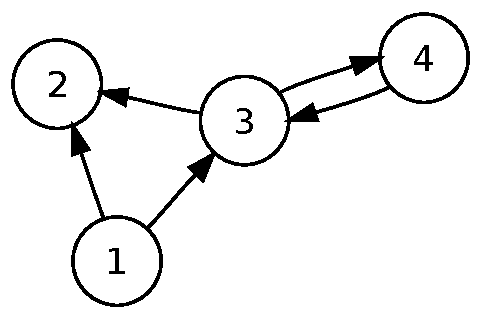
\includegraphics[width=.8\linewidth]{assets/images/Directed_graph_no_background.svg.pdf}
            \caption{Directed graph with cycle between nodes three and four.}
            \label{fig:directedgraph}
        \end{subfigure}
        \begin{subfigure}{.5\textwidth}
            \centering
            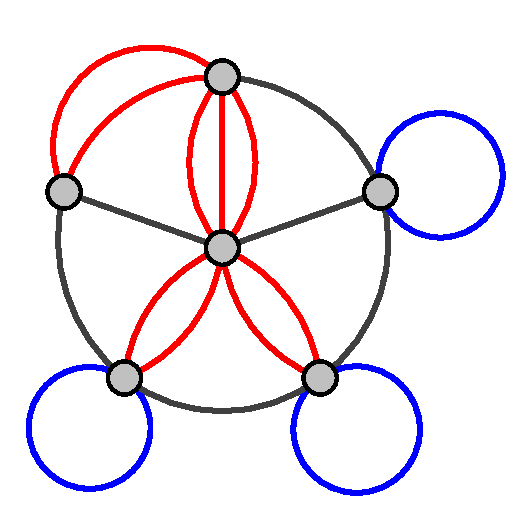
\includegraphics[width=.8\linewidth]{assets/images/Multi-pseudograph.svg.pdf}
            \caption{Multigraph with parallel edges and self-loops}
            \label{fig:multigraph}
        \end{subfigure}%
        \caption[]{Examples of first order graph symantics supported by Jaseci.\footnotemark}
        \label{fig:graph_examples}
    \end{figure}
    \footnotetext{Images credits to wiki contributers~\cite{wiki:Directed_graph_no_background.svg,wiki:Multi-pseudograph.svg}}
}


\newcommand{\printfigHelloWorldBaby}{
    \begin{figure}%{r}{0.5\textwidth}
        \centering
        
\includegraphics[width=.3\linewidth]{assets/images/hello_world_baby.jpg}
        \caption[]{World's youngest coder with valid HTML on shirt.\footnotemark}
        \label{fig:hello_baby}
    \end{figure}
    \footnotetext{Image credit to wiki contributer~\cite{wiki:hello_world_baby.jpg}}
}

\newcommand{\printtabPrecedence}{
    \begin{table}[t]
        \footnotesize
        \centering
        \begin{tabular}{l l l}
            \toprule
            \textbf{Rank} & \textbf{Symbol}                            & \textbf{Description}                           \\
            \midrule
            1             & \texttt{( ), [ ], ., ::, spawn}            & Parenthetical/grouping, node/edge manipulation \\
            2             & \texttt{\textasciicircum, []}              & Exponent,  Index                               \\
            3             & \texttt{*, /, \%  }                        & Multiplication, division, modulo               \\
            4             & \texttt{+, -}                              & Addition, subtraction                          \\
            5             & \texttt{==, !=, >=, <=, >, <, in, not in } & Comparison                                     \\
            6             & \texttt{\&\&, ||, and, or  }               & Logical                                        \\
            7             & \texttt{-->, <--, -[]->, <-[]-}            & Connect                                        \\
            8             & \texttt{=, +=, -=, *=, /=, := }            & Assignment                                     \\
            \bottomrule
        \end{tabular}
        \caption{Precedence of operations in Jac}
        \label{tab:jacprecedence} % Unique label used for referencing the table in-text
        %\addcontentsline{toc}{table}{Table \ref{tab:jacprecedence}} % Uncomment to add the table to the table of contents
    \end{table}
}

\newcommand{\printtabStrOps}{
    \begin{table}[t]
        \footnotesize
        \centering
        \rowcolors{1}{light-cyan}{light-gray}
        \begin{tabular}{l p{3cm} p{6cm}}
            \toprule
            \textbf{Op}                                           & \textbf{Args}                                                                                                                                                  & \textbf{Description} \\
            \midrule
            \lstinline{.str::upper}                               & none                                                                                                                                                           &                      \\
            \lstinline{.str::lower}                               & none                                                                                                                                                           &                      \\
            \lstinline{.str::title}                               & none                                                                                                                                                           &                      \\
            \lstinline{.str::capitalize}                          & none                                                                                                                                                           &                      \\
            \lstinline{.str::swap\_case}                          & none                                                                                                                                                           &                      \\
            \lstinline{.str::is\_alnum}                           & none                                                                                                                                                           &                      \\
            \lstinline{.str::is\_digit}                           & none                                                                                                                                                           &                      \\
            \lstinline{.str::is\_title}                           & none                                                                                                                                                           &                      \\
            \lstinline{.str::is\_upper}                           & none                                                                                                                                                           &                      \\
            \lstinline{.str::is\_lower}                           & none                                                                                                                                                           &                      \\
            \lstinline{.str::is\_space}                           & none                                                                                                                                                           &                      \\
            \lstinline{.str::load\_json}                          & none                                                                                                                                                           &                      \\
            \lstinline{.str::count}      & (\textbf{substr}, start, end)            & Returns the number of occurrences of a substring in the given string. Start and end specify range of indices to search                                                                \\
            \lstinline{.str::find}       &   (\textbf{substr}, start, end)            & Returns the index of first occurrence of the substring (if found). If not found, it returns -1. Start and end specify range of indices to search.                                     \\
            \lstinline{.str::split}      & \emph{optional} (separator, maxsplit) & Breaks up a string at the specified separator for maxsplit number of times and returns a list of strings. Default separators is ` ' and maxsplit is unlimited.                        \\
            \lstinline{.str::startswith}                          &                                                                                                                                                                &                      \\
            \lstinline{.str::endswith}                            &                                                                                                                                                                &                      \\
            \lstinline{.str::replace}                             &                                                                                                                                                                &                      \\
            \lstinline{.str::strip}                               & optional,                                                                                                                                                      &                      \\
            \lstinline{.str::lstrip}                              & optional,                                                                                                                                                      &                      \\
            \lstinline{.str::rstrip}                              & optional,                                                                                                                                                      &                      \\
            \bottomrule
        \end{tabular}
        \caption{String operations in Jac}
        \label{tab:strops} % Unique label used for referencing the table in-text
        %\addcontentsline{toc}{table}{Table \ref{tab:jacprecedence}} % Uncomment to add the table to the table of contents
    \end{table}
}

\newcommand{\printtabListOps}{
    \begin{table}[t]
        \footnotesize
        \centering
        \begin{tabular}{l l l}
            \toprule
            \textbf{Op}                     & \textbf{Args} & \textbf{Description}               \\
            \midrule
            \lstinline{.list::max}          & none          &                                    \\
            \lstinline{.list::min}          & none          &                                    \\
            \lstinline{.list::idx\_of\_max} & none          &                                    \\
            \lstinline{.list::idx\_of\_min} & none          &                                    \\
            \lstinline{.list::copy}         & none          & Returns a shallow copy of the list \\
            \lstinline{.list::deepcopy}     & none          & Returns a deep copy of the list    \\
            \lstinline{.list::sort}         & none          &                                    \\
            \lstinline{.list::reverse}      & none          &                                    \\
            \lstinline{.list::clear}        & none          &                                    \\
            \lstinline{.list::pop}          & optional,     &                                    \\
            \lstinline{.list::index}        &               &                                    \\
            \lstinline{.list::append}       &               &                                    \\
            \lstinline{.list::extend}       &               &                                    \\
            \lstinline{.list::insert}       &               &                                    \\
            \lstinline{.list::remove}       &               &                                    \\
            \lstinline{.list::count}        &               &                                    \\
            \bottomrule
        \end{tabular}
        \caption{List operations in Jac}
        \label{tab:listops} % Unique label used for referencing the table in-text
        %\addcontentsline{toc}{table}{Table \ref{tab:jacprecedence}} % Uncomment to add the table to the table of contents
    \end{table}
}

\newcommand{\printtabDictOps}{
    \begin{table}[t]
        \footnotesize
        \centering
        \begin{tabular}{l l l}
            \toprule
            \textbf{Op}                 & \textbf{Args} & \textbf{Description}                     \\
            \midrule
            \lstinline{.dict::items}    & none          &                                          \\
            \lstinline{.dict::copy}     & none          & Returns a shallow copy of the dictionary \\
            \lstinline{.dict::deepcopy} & none          & Returns a deep copy of the dictionary    \\
            \lstinline{.dict::keys}     & none          &                                          \\
            \lstinline{.dict::clear}    & none          &                                          \\
            \lstinline{.dict::popitem}  & none          &                                          \\
            \lstinline{.dict::values}   & none          &                                          \\
            \lstinline{.dict::pop}      &               &                                          \\
            \lstinline{.dict::update}   &               &                                          \\
            \bottomrule
        \end{tabular}
        \caption{Dictionary operations in Jac}
        \label{tab:dictops} % Unique label used for referencing the table in-text
        %\addcontentsline{toc}{table}{Table \ref{tab:jacprecedence}} % Uncomment to add the table to the table of contents
    \end{table}
}

\newcommand{\printtabJSAPI}{
    \rowcolors{1}{light-cyan}{light-gray}
    \begin{longtable}{l | p{10cm}}
        \toprule
        \rowcolor{white} \textbf{Interface} & \textbf{Parameters} \\
        \midrule
        \lstinline$walker summon$ & \lstinline$key: str (*req), wlk: walker (*req), nd: node (*req), ctx: dict (\{\}), _req_ctx: dict (\{\}), global_sync: bool (True)$ \\ \hline
\lstinline$walker callback$ & \lstinline$nd: node (*req), wlk: walker (*req), key: str (*req), ctx: dict (\{\}), _req_ctx: dict (\{\}), global_sync: bool (True)$ \\ \hline
\lstinline$walker register$ & \lstinline$snt: sentinel (None), code: str (), encoded: bool (False)$ \\ \hline
\lstinline$walker get$ & \lstinline$wlk: walker (*req), mode: str (default), detailed: bool (False)$ \\ \hline
\lstinline$walker set$ & \lstinline$wlk: walker (*req), code: str (*req), mode: str (default)$ \\ \hline
\lstinline$walker list$ & \lstinline$snt: sentinel (None), detailed: bool (False)$ \\ \hline
\lstinline$walker delete$ & \lstinline$wlk: walker (*req), snt: sentinel (None)$ \\ \hline
\lstinline$walker spawn create$ & \lstinline$name: str (*req), snt: sentinel (None)$ \\ \hline
\lstinline$walker spawn list$ & \lstinline$detailed: bool (False)$ \\ \hline
\lstinline$walker spawn delete$ & \lstinline$name: str (*req)$ \\ \hline
\lstinline$walker spawn clear$ & \lstinline$n/a$ \\ \hline
\lstinline$walker yield list$ & \lstinline$detailed: bool (False)$ \\ \hline
\lstinline$walker yield delete$ & \lstinline$name: str (*req)$ \\ \hline
\lstinline$walker yield clear$ & \lstinline$n/a$ \\ \hline
\lstinline$walker prime$ & \lstinline$wlk: walker (*req), nd: node (None), ctx: dict (\{\}), _req_ctx: dict (\{\})$ \\ \hline
\lstinline$walker execute$ & \lstinline$wlk: walker (*req), prime: node (None), ctx: dict (\{\}), _req_ctx: dict (\{\}), profiling: bool (False)$ \\ \hline
\lstinline$walker run$ & \lstinline$name: str (*req), nd: node (None), ctx: dict (\{\}), _req_ctx: dict (\{\}), snt: sentinel (None), profiling: bool (False)$ \\ \hline
\lstinline$user create$ & \lstinline$name: str (*req), global_init: str (), global_init_ctx: dict (\{\}), other_fields: dict (\{\})$ \\ \hline
\lstinline$alias register$ & \lstinline$name: str (*req), value: str (*req)$ \\ \hline
\lstinline$alias list$ & \lstinline$n/a$ \\ \hline
\lstinline$alias delete$ & \lstinline$name: str (*req)$ \\ \hline
\lstinline$alias clear$ & \lstinline$n/a$ \\ \hline
\lstinline$global get$ & \lstinline$name: str (*req)$ \\ \hline
\lstinline$global set$ & \lstinline$name: str (*req), value: str (*req)$ \\ \hline
\lstinline$global delete$ & \lstinline$name: str (*req)$ \\ \hline
\lstinline$global sentinel set$ & \lstinline$snt: sentinel (None)$ \\ \hline
\lstinline$global sentinel unset$ & \lstinline$n/a$ \\ \hline
\lstinline$object get$ & \lstinline$obj: element (*req), depth: int (0), detailed: bool (False)$ \\ \hline
\lstinline$object perms get$ & \lstinline$obj: element (*req)$ \\ \hline
\lstinline$object perms set$ & \lstinline$obj: element (*req), mode: str (*req)$ \\ \hline
\lstinline$object perms default$ & \lstinline$mode: str (*req)$ \\ \hline
\lstinline$object perms grant$ & \lstinline$obj: element (*req), mast: element (*req), read_only: bool (False)$ \\ \hline
\lstinline$object perms revoke$ & \lstinline$obj: element (*req), mast: element (*req)$ \\ \hline
\lstinline$graph create$ & \lstinline$set_active: bool (True)$ \\ \hline
\lstinline$graph get$ & \lstinline$gph: graph (None), mode: str (default), detailed: bool (False)$ \\ \hline
\lstinline$graph list$ & \lstinline$detailed: bool (False)$ \\ \hline
\lstinline$graph active set$ & \lstinline$gph: graph (*req)$ \\ \hline
\lstinline$graph active unset$ & \lstinline$n/a$ \\ \hline
\lstinline$graph active get$ & \lstinline$detailed: bool (False)$ \\ \hline
\lstinline$graph delete$ & \lstinline$gph: graph (*req)$ \\ \hline
\lstinline$graph node get$ & \lstinline$nd: node (*req), keys: list ([])$ \\ \hline
\lstinline$graph node set$ & \lstinline$nd: node (*req), ctx: dict (*req), snt: sentinel (None)$ \\ \hline
\lstinline$graph walk (cli only)$ & \lstinline$nd: node (None)$ \\ \hline
\lstinline$sentinel register$ & \lstinline$name: str (default), code: str (), code_dir: str (./), mode: str (default), encoded: bool (False), auto_run: str (init), auto_run_ctx: dict (\{\}), auto_create_graph: bool (True), set_active: bool (True)$ \\ \hline
\lstinline$sentinel pull$ & \lstinline$set_active: bool (True), on_demand: bool (True)$ \\ \hline
\lstinline$sentinel get$ & \lstinline$snt: sentinel (None), mode: str (default), detailed: bool (False)$ \\ \hline
\lstinline$sentinel set$ & \lstinline$code: str (*req), code_dir: str (./), encoded: bool (False), snt: sentinel (None), mode: str (default)$ \\ \hline
\lstinline$sentinel list$ & \lstinline$detailed: bool (False)$ \\ \hline
\lstinline$sentinel test$ & \lstinline$snt: sentinel (None), detailed: bool (False)$ \\ \hline
\lstinline$sentinel active set$ & \lstinline$snt: sentinel (*req)$ \\ \hline
\lstinline$sentinel active unset$ & \lstinline$n/a$ \\ \hline
\lstinline$sentinel active global$ & \lstinline$auto_run: str (), auto_run_ctx: dict (\{\}), auto_create_graph: bool (False), detailed: bool (False)$ \\ \hline
\lstinline$sentinel active get$ & \lstinline$detailed: bool (False)$ \\ \hline
\lstinline$sentinel delete$ & \lstinline$snt: sentinel (*req)$ \\ \hline
\lstinline$wapi$ & \lstinline$name: str (*req), nd: node (None), ctx: dict (\{\}), _req_ctx: dict (\{\}), snt: sentinel (None), profiling: bool (False)$ \\ \hline
\lstinline$architype register$ & \lstinline$code: str (*req), encoded: bool (False), snt: sentinel (None)$ \\ \hline
\lstinline$architype get$ & \lstinline$arch: architype (*req), mode: str (default), detailed: bool (False)$ \\ \hline
\lstinline$architype set$ & \lstinline$arch: architype (*req), code: str (*req), mode: str (default)$ \\ \hline
\lstinline$architype list$ & \lstinline$snt: sentinel (None), detailed: bool (False)$ \\ \hline
\lstinline$architype delete$ & \lstinline$arch: architype (*req), snt: sentinel (None)$ \\ \hline
\lstinline$master create$ & \lstinline$name: str (*req), global_init: str (), global_init_ctx: dict (\{\}), other_fields: dict (\{\})$ \\ \hline
\lstinline$master get$ & \lstinline$name: str (*req), mode: str (default), detailed: bool (False)$ \\ \hline
\lstinline$master list$ & \lstinline$detailed: bool (False)$ \\ \hline
\lstinline$master active set$ & \lstinline$name: str (*req)$ \\ \hline
\lstinline$master active unset$ & \lstinline$n/a$ \\ \hline
\lstinline$master active get$ & \lstinline$detailed: bool (False)$ \\ \hline
\lstinline$master self$ & \lstinline$detailed: bool (False)$ \\ \hline
\lstinline$master delete$ & \lstinline$name: str (*req)$ \\ \hline
\lstinline$master createsuper$ & \lstinline$name: str (*req), global_init: str (), global_init_ctx: dict (\{\}), other_fields: dict (\{\})$ \\ \hline
\lstinline$master allusers$ & \lstinline$num: int (0), start_idx: int (0)$ \\ \hline
\lstinline$master become$ & \lstinline$mast: master (*req)$ \\ \hline
\lstinline$master unbecome$ & \lstinline$n/a$ \\ \hline
\lstinline$config get$ & \lstinline$name: str (*req), do_check: bool (True)$ \\ \hline
\lstinline$config set$ & \lstinline$name: str (*req), value: str (*req), do_check: bool (True)$ \\ \hline
\lstinline$config list$ & \lstinline$n/a$ \\ \hline
\lstinline$config index$ & \lstinline$n/a$ \\ \hline
\lstinline$config exists$ & \lstinline$name: str (*req)$ \\ \hline
\lstinline$config delete$ & \lstinline$name: str (*req), do_check: bool (True)$ \\ \hline
\lstinline$logger http connect$ & \lstinline$host: str (*req), port: int (*req), url: str (*req), log: str (all)$ \\ \hline
\lstinline$logger http clear$ & \lstinline$log: str (all)$ \\ \hline
\lstinline$logger list$ & \lstinline$n/a$ \\ \hline
\lstinline$actions load local$ & \lstinline$file: str (*req)$ \\ \hline
\lstinline$actions load remote$ & \lstinline$url: str (*req)$ \\ \hline
\lstinline$actions load module$ & \lstinline$mod: str (*req)$ \\ \hline
\lstinline$actions list$ & \lstinline$name: str ()$ \\ \hline
\lstinline$jac build (cli only)$ & \lstinline$file: str (*req), out: str ()$ \\ \hline
\lstinline$jac test (cli only)$ & \lstinline$file: str (*req), detailed: bool (False)$ \\ \hline
\lstinline$jac run (cli only)$ & \lstinline$file: str (*req), walk: str (init), ctx: dict (\{\}), profiling: bool (False)$ \\ \hline
\lstinline$jac dot (cli only)$ & \lstinline$file: str (*req), walk: str (init), ctx: dict (\{\}), detailed: bool (False)$ \\ \hline

        \bottomrule
        \hiderowcolors
        \caption{Full set of core Jaseci APIs}
        \label{tab:jsAPI}
    \end{longtable}
}
\newglossaryentry{christen}
{
    name=christen,
    description={to name or dedicate (something, such as a piece of code) by a ceremony that often involves breaking a bottle of champagne}
}
\newglossaryentry{pwn}
{
    name=pwn,
    description={the act of dominating a person, place, or thing. (...or a piece of code)}
}

\newglossaryentry{gobbledygook}
{
    name=gobbledygook,
    description={language that is meaningless or is made unintelligible by excessive use of abstruse technical terms; nonsense}
}
\newglossaryentry{bleh}
{
    name=bleh,
    description={mildly yucky}
}
\newglossaryentry{leet}
{
    name=leet,
    description={v. hyper-sophisticated from a coding perspective, n. a language used by \gls{leet} \gls{haxor}s}
}

\newglossaryentry{haxor}
{
    name=haxor,
    description={\gls{leet} spelling of hacker}
}
\newglossaryentry{coder}
{
    name=coder,
    description={the superior human}
}
\newglossaryentry{Jaseci jolt}
{
    name=Jaseci jolt,
    description={an insight derived from Jaseci that serves as a high voltage bolt of energy to the mind of a sharp coder.}
}
\newglossaryentry{common languages}
{
    name=common languages,
    description={typical languages programmers use to write commercial software, (e.g., C, C++, Java, Javascript, Python, Ruby, Go, Perl, PHP, etc.)}
}

\newglossaryentry{grok}
{
    name=grok,
    description={to fully comprehend and understand deeply }
}

\newglossaryentry{sick}
{
    name=sick,
    description={\gls{redonkulous}}
}

\newglossaryentry{redonkulous}
{
    name=redonkulous,
    description={\gls{dope}}
}

\newglossaryentry{dope}
{
    name=dope,
    description={\gls{sick}}
}

\newglossaryentry{goo goo gaa gaa}
{
    name=goo goo gaa gaa,
    description={the language of babies}
}

\newglossaryentry{directed graphs}
{
    type=technical,
    name=directed graphs,
    description={a directed graph (or digraph) is a graph that is made up of a set of vertices connected by directed edges (think edges as arrows as opposed to lines) often called arcs}
}
\newglossaryentry{undirected graphs}
{
    type=technical,
    name=undirected graphs,
    description={a graph made up of vertices (also called nodes or points) which are connected symmetrically by edges (also called links or lines)}
}

\newglossaryentry{multigraphs}
{
    type=technical,
    name=multigraph,
    description={a graph which is permitted to have multiple edges (also called parallel edges[1]), that is, edges that have the same end nodes}
}

\newglossaryentry{hypergraphs}
{
    type=technical,
    name=hypergraph,
    description={a hypergraph is a generalization of a graph in which an edge can join any number of vertices in contrast to connecting exactly two vertices}
}

\newglossaryentry{contexts}
{
    type=technical,
    name=contexts,
    description={A set of key value pairings that serve as a data payload attributable to nodes and edges in Jaseci graphs}
}

\newglossaryentry{walker}
{
    type=technical,
    name=walker,
    description={An abstraction in the Jaseci machine and Jac programming language that represents a computational agent that computes and travels along nodes and edges of a graph}
}

\newglossaryentry{sentinel}
{
    type=technical,
    name=sentinel,
    description={Overseer of walkers and architype nodes and edges.}
}
\newglossaryentry{IMHO}
{
    name=IMHO,
    description={Acronym for ``In My Humble Opinion''}
}

\newglossaryentry{WSL}
{
    type=technical,
    name=WSL,
    description={Windows Subsystem for Linux}
}
\newglossaryentry{dynamically typed language}
{
    type=technical,
    name=dynamically typed language,
    description={a language is dynamically typed if the type is associated with run-time values, and not named variables/fields/etc. This means that a programmer can code a bit quicker not having to specify types statically.}
}

\begin{document}


\def\JJ{JASECI} % Title
\def\BB{BIBLE} % Title
\title{\JJ \BB}

\def\Me{Jason Mars, \xout{PhD} Ninja} % Author
\author\Me

\def\VER{v1.3}
\definecolor{title_white}{rgb}{1,1,1}
\definecolor{title_grey}{rgb}{0.6,0.6,0.6}


\newpagecolor{black}
\vspace{\fill}
\addtolength{\topmargin}{1in}



\setstretch{10.0}


\begingroup
\bf\centering
{\color{title_white} \scalebox{4}[4]{\JJ}}\\
{\color{title_grey} \scalebox{7}[7]{\BB}}\\
{\color{title_white} \scalebox{2}[2]{\Me}}\par
{\color{title_white} \scalebox{2}[2]{\VER}}
\endgroup


\pagebreak
\restorepagecolor
\thispagestyle{empty}
%After title we restore all margins.
\newgeometry{margin=1in}
\setstretch{1.0}



\newpagecolor{black}
\vspace{\fill}
\addtolength{\topmargin}{1.5in}



\setstretch{2.0}


\begingroup
\bf
\color{white}\LARGE

% Warning: This book is a trigger factory.
% \vspace{1in}
% \par \Large \setstretch{1.0}
% If after reading that sentence you feel a sense of concern, this book WILL trigger you and you'll need to refer to the previous page and continue. If you are not concerned after reading the warning, continue with caution.
\par \Large \setstretch{1.0}
I welcome you, neophyte, to embark on the journey of becoming a true Jaseci Ninja!

\par\small
Btw, this is a silly book in places, please take that seriously :-)
\endgroup


\pagebreak
\restorepagecolor

%After title we restore all margins.
\newgeometry{margin=1in}
\setstretch{1.0}

\normalem
\cleardoublepage % Make toc appear on right side.
\setcounter{secnumdepth}{3} % toc is 2 level deep.
\dominitoc
\tableofcontents
\pagebreak
\printglossary[title=Not So Technical Terms Used, toctitle=List of Terms]
\printglossary[type=technical, title=Technical Terms Used, toctitle=List of Technical Terms]
\mtcaddchapter
\mtcaddchapter
\mtcaddchapter


\chapter*{Preface}
\addcontentsline{toc}{chapter}{Preface}

The way we design and write software to do computation and AI today is poop. How poopy you ask? Hrm\dots, let me think\dots, In my approximation, if you were to use it as a fuel source, it would be able to run all the blockchain transactions across the aggregate of current and future coins for a decade.
\par
Hrm, too much? Probably. I guess you'd expect me to use concrete examples and cite evidence to make my points. I mean, I could write something like \textit{``The imperative programming model utilized in near all of the production software produced in the last four decades has not fundamentally changed since blah blah blah..."}. I'd certainly sound more credible and such. Well, though I have indeed grown accustomed to writing that way, boy has it gotten old.
\par
I'm not going to do that for this book. Let's have fun. After all, Jaseci has never been work for me, its play (and art). Very ambitious play granted, but play at it's core.
\par
Everything here is based on my opinion\dots no, expert \emph{ninja} opinion, and my intuition. That suffices for me, and I hope it does for you. Even though I have spent decades coding and leading teams of coders working on the holy grail technical challenges of our time, I won't rely on that to assert credibility. Lets let these ideas stand or die on their own merit. Its my gut that tells me that we can do better. This book describes my attempt at better. I hope you find value in it. If you do, awesome! If you don't, awesome!


\chapter{Introduction}
Coming Soon...




\part{World of Jaseci}
\label{part:jsword}
\chapter{What and Why is Jaseci?}
\minitoc
\section{TL;DR}
Modern production applications are \emph{diffuse}, spanning multiple individual programs (database, memcache, logging, application logic, AI models, etc) interfacing each other over APIs to realize a single product functionality.
        Creating such applications at scale is technically challenging, requires a highly-skilled developer team, is rife with complexity, and is, for many, prohibitively costly.
        This complexity is in stark contrast to the era of computing where a state of the art software product was a single binary that ran on one machine and could be developed by a single programmer.
        Though a number of important abstractions and technologies have emerged to help mitigate this complexity, the creation of sophisticated production software in practices is still highly complex and requires a team of engineers.


        In this work, the case is made for a wholistic top-down re-envisioning of the system stack from the programming language level down through the system architecture to bridge this complexity gap.
        The key goal of our design is to address the critical need for the programmer to articulate solutions with higher level abstractions at the problem level while having the runtime system stack subsume and hide a broad scope of diffuse sub-applications and inter-machine resources.
        This work also presents the design of a production-grade realization of such a system stack architecture called \textbf{Jaseci}, and corresponding programming language \textbf{Jac}.
        Jac and Jaseci has been released as open source and has been leveraged by real product teams to accelerate developing and deploying sophisticated AI products and other applications at scale.
        Jac has been utilized in commercial production environments to accelerate AI development timelines by  $\sim$10x, with the Jaseci runtime automating the decisions and optimizations typically falling in the scope of manual engineering roles on a team such as what should and should not be a microservice and changing those dynamically.
\section{Introduction and Motivation}
There has been a fundamental paradigm shift in the landscape of how we build software over the last 2 decades.
The compute stack was originally envisaged with the assumption that a single program would run on a single machine.
In this traditional model, system software abstractions subsumed the management of processor, memory, disk and physically connected peripherals within the context of the machine.
However, this landscape rapidly changed with the evolution toward software being served on the backbone provided by the internet.
Now, an `application' is realized through the cooperation of multiple distinct sub-applications (services) running collaboratively.
For example a single application my contain self one or more self-contained database, memcache, logging, application logic, AI model applications interfacing each other over APIs as shown in Figure~\ref{fig:intro} (left).
We call these applications \emph{diffuse applications}.


This work contends that the fundamental programming paradigms in computing has not evolved at pace.
The abstractions envisioned during the era of the single machine computational model is still present at the programming interface and throughout the runtime stack leading to significant and costly complexity.


To address this complexity, two keystone abstractions have recently emerged to facilitate the development of these diffuse applications.
The first of these abstractions is the introduction and rapid dissemination of containerization service platforms.
With what started as a key insight articulated in ``The Datacenter as a Computer,'' Google would innovate their Borg system and ultimately released it open source as Kubernetes.
With Kubernetes, the underlying hardware resources would be abstracted away with the introduction of \emph{pods} (virtual machines), and other resources that can be virtually networked together and otherwise configured irrespective of the physical hardware.
Today, Kubernetes is the most prevalent containerized service abstraction layer in cloud computing.
The second of keystone abstraction would be coined ``Severless Computing'' and gained prominence with the introduction of Amazons Lamda functions.
This FaaS abstraction would facilitate the development of diffuse applications at the level of functions and abstract away the underlying containerized service ecosystem.
A programer can simply make function calls in their favorite language without every needing to be aware of where the function will run nor the system level resources that would be allocated or managed.

\begin{figure}[tb]
    \centering
    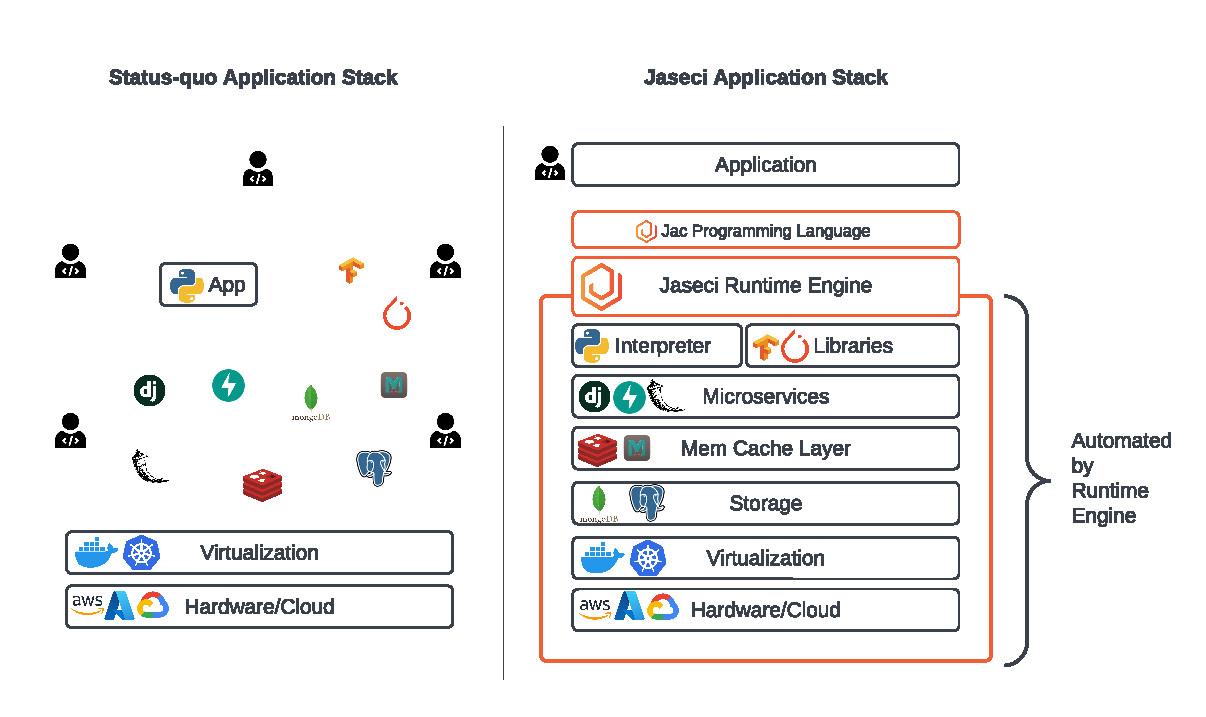
\includegraphics[width=\linewidth]{figures/jaseci_stack.pdf}
    \caption{Comparison between status quo development of production grade \emph{diffuse} applications (left), and the Jaseci technology stack that hides and automates an expanded set of subsystems through raising the level of abstraction (right).}
    \label{fig:intro}
\end{figure}



Though these two abstractions have been highly impactful, these innovations in our stack architecture represent a bottom up evolution of abstractions.
As a result, programmers are still left with single-machine abstractions at the programming interface and must grapple with a significant amount of complexity.
For example, traditional languages and their runtime stacks are predominately designed with the goal of hiding and managing intra-machine resources while what is needed for diffuse applications is the hiding and management of inter-machine resources.
Analogous to the virtualization and management of allocated memory on the heap provided by garbage collectors in modern languages (intra-machine), the virtualization and management of resources such as microservice creation, scheduling and orchestration alongside policies for organizing distributed databases, mem caches, logging and other highly complex subsystems (inter-machine) is not only needed, but as we show in this work, possible and practical.
Without this raising of the level of abstraction, it has become prohibitively difficult for a single engineer to invent, build, deploy, launch, and scale modern cutting edge applications.

To the best of our knowledge, we are not aware of a thorough, wholistic, and top-down design of a serverless programming paradigm and computational stack from the language level down through the system runtime stack to hide this expanded set of resources.

In this work, we present a wholistic design approach with the goal of abstracting away and automating a new class of underlying systems, allowing a programmer to articulate solutions and diffuse applications at the problem level.
We present the design of a \emph{diffuse runtime execution engine} we call \textbf{Jaseci}, and a \emph{data-spacial programming language} we call \textbf{Jac}.

The design of Jaseci and Jac has initially been inspired to by sophisticated emerging AI applications at scale and is driven by two key insightss.

\begin{itemize}

    \item \emph{Higher level abstractions are needed at the language level to allow single creators to work at the problem level to build end-to-end diffuse AI products.}
    \item \emph{A new set of abstractions across the language runtime and system stack is needed to automate and hide the class of inter-machine resources from the programmer.}

\end{itemize}

\noindent
To this end we present techniques across two categories,

\begin{enumerate}


    \item \emph{Jac Language} - A language that introduces a new set of abstractions, namely \textbf{data-spacial scoping} and \textbf{agent oriented programming}. These abstractions natively facilitates the emerging need to reason about and solve problems with graph representations as well as the need for algorithmic modularity and encapsulation to hide a new class of inter-machine resources.
    \item \emph{Jaseci Diffuse Runtime Engine} - A runtime that raises the abstraction layer to the problem solving level where the runtime engine subsumes responsibility for not only for the optimization of program code, but the orchestration, configuration, and optimization of the full cloud compute stack and inter-machine resources (such tasks as container formation, scaling and optimization).


\end{enumerate}


Jaseci and Jac is fully functional, open-source~\cite{jaseci-website,jaseci-github,jaseci-pypi}, and used in production for four real-world products today.
These commercial products were built entirely on the Jaseci staci and includes Myca~\cite{myca-website}, HomeLendingPal~\cite{hlp-website},  ZeroShotBot~\cite{zsb-website} and TrueSelph~\cite{ts-website}.
Across these and other projects, the Jac language has been used by dozens of programmers in the creation of production software and Jaseci deployments support tens of thousands of production queries per day currently.
In practice, our initial infrastructure has been leveraged in practice to achieve 10x reduction in development time and near 100\% elimination of typical backend code needed for a complicated AI based application.

The specific contributions of this paper include:
\begin{itemize}
    \item We formulate the problem of development complexity and present a top down programing paradigm and runtime stack for diffuse applications.
    \item We describe the design and implementation Jaseci's \textbf{diffuse runtime execution engine}.
    \item We introduce Jac, a language that implements a \textbf{data-spacial} programming paradigm (the first of its kind).
    \item We describe the utility of Jaseci and Jac through real world case studies of building out a real production scale-out product.
\end{itemize}

We find that the wholistic design philosophy and resulting paradigm of Jaseci and Jac is a promising one.
Multiple development teams have adopted the data spacial programming model of Jac and the diffuse runtime execution engine in Jaseci to build sophisticated AI products with significantly reduced complexity and teaming.
\section{The Case for Change}
Though recent advancements in serverless computing has been instrumental in improving the ability of teams to more rapidly develop software, significant challenges remain in the development of cutting edge applications and products in our current compute landscape.
An demonstrative problem domain with this challenge are those characterized by applications that include sophisticated AI pipelines on their critical path.

\begin{figure}[tb]
    \centering
    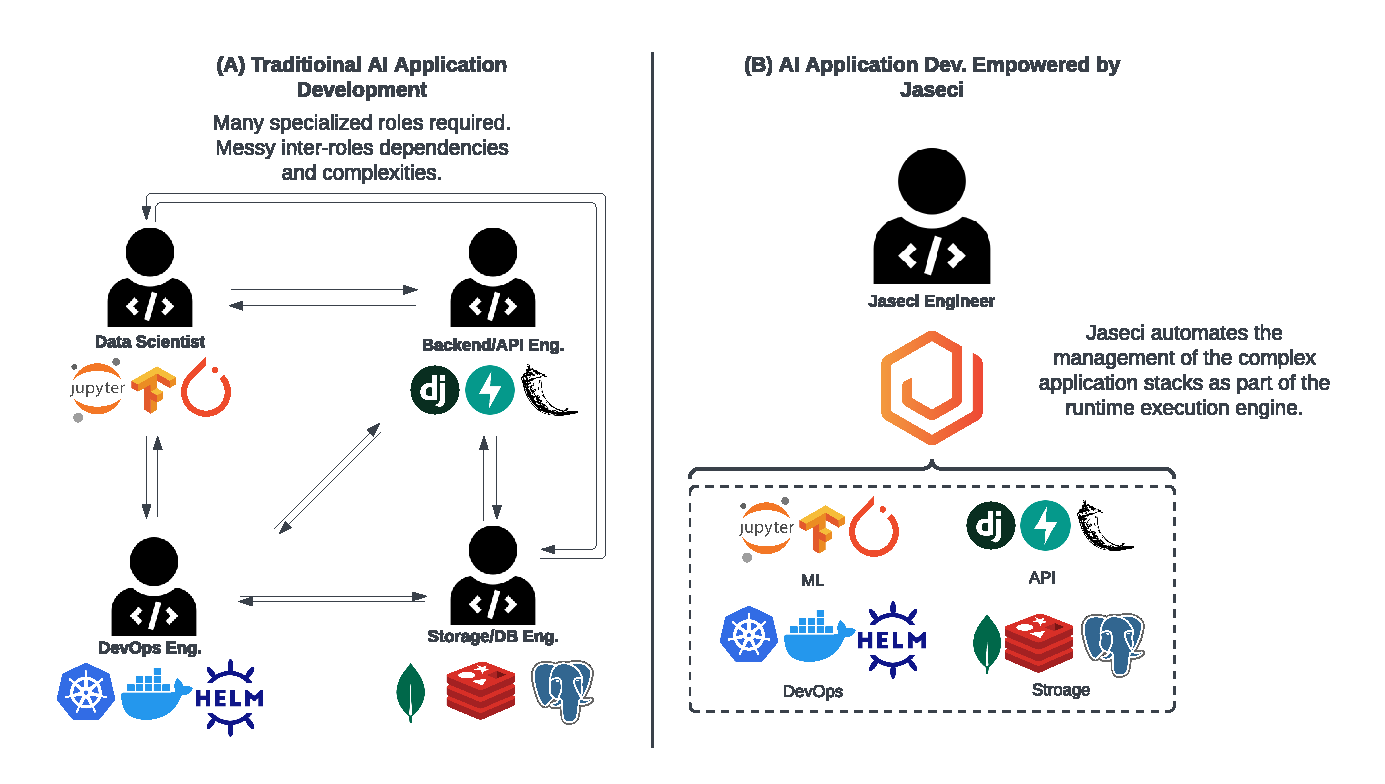
\includegraphics[width=\linewidth]{figures/team_sizes.pdf}
    \caption{Comparison of typical development team required to realize production grade AI application today (left), and the ability of a single software developer to realize such an application with Jaseci (right). }
    \label{fig:dev}
\end{figure}


\subsection{Problem Scenario}
Figure~\ref{fig:dev}A shows the typical set of  often siloed roles needed to create software in this environment.
The first critical role needed is an \emph{architect / tech-lead} responsible for architecting the software solution across disparate components, programming languages, frameworks, and SDKs.
If a microservice ecosystem is needed (which is a must for modern
AI applications), the architect will also decide what will and won't be its own service (container) and define the interfaces between these disparate  services.
For the AI model work, the role of a \emph{data scientist / ML engineer} is needed.
This role typically works primarily in Jupyter notebooks selecting, creating, training and tuning ML models to support application features.
Production software engineering is typically outside of the scope of this expertise in practice.
The role of a \emph{backend engineer} is needed for implementing the main services of the application and taking the code out of Jupyter notebooks to build the models into the backend (server-side) of the application.
The \emph{backend engineer} is also responsible for supporting new features and creating their API interfaces for \emph{frontend} engineers.
One of the key roles any software team needs to deploy an AI product is a \emph{DevOps engineer}.
This role is solely responsible for deploying and configuring containers to run on a cloud and ensure these containers are operational and scaled to the load requirements of the software.
This responsibility covers configuring software instance pods, database pods, caching layers, logging services, and parameterizing replicas and auto-scaling heuristics.



In this traditional model of software engineering, many challenges and complexity emerge.
An example is the (quite typical) scenario of the first main server-side implementation of the application being a monoservice while DB, caching, and logging are microservices.
As the \emph{ML engineer} introduces models of increasing size, the \emph{dev-ops} person alerts the team that the cloud instances, though designated as \emph{large}, only have 8gb of ram.
Meanwhile new AI models being integrated exceed this limit.
This event leads to a re-architecture of the main monoservice to be split out AI models into microservices and interfaces being designed or adopted leading to significant backend work / delays.
In this work, we aim to create a solution that would move all of this decisioning and work under the purview of the automated runtime system.

Ultimately, the mission of Jaseci is to accelerate and democratize the development and deployments of end-to-end scalable AI applications as presented in Figure~\ref{fig:dev}B.
To this end, we present a novel set of higher level abstractions for programming sophisticated software in a micro-service/serverless AI and a full stack architecture and programming model that abstracts away and automates much of the complexity of building diffuse applications on a distributed compute substrate of potentially thousands of compute nodes.
\section{A Higher Level Language}
\begin{figure}[tb]
    \centering
    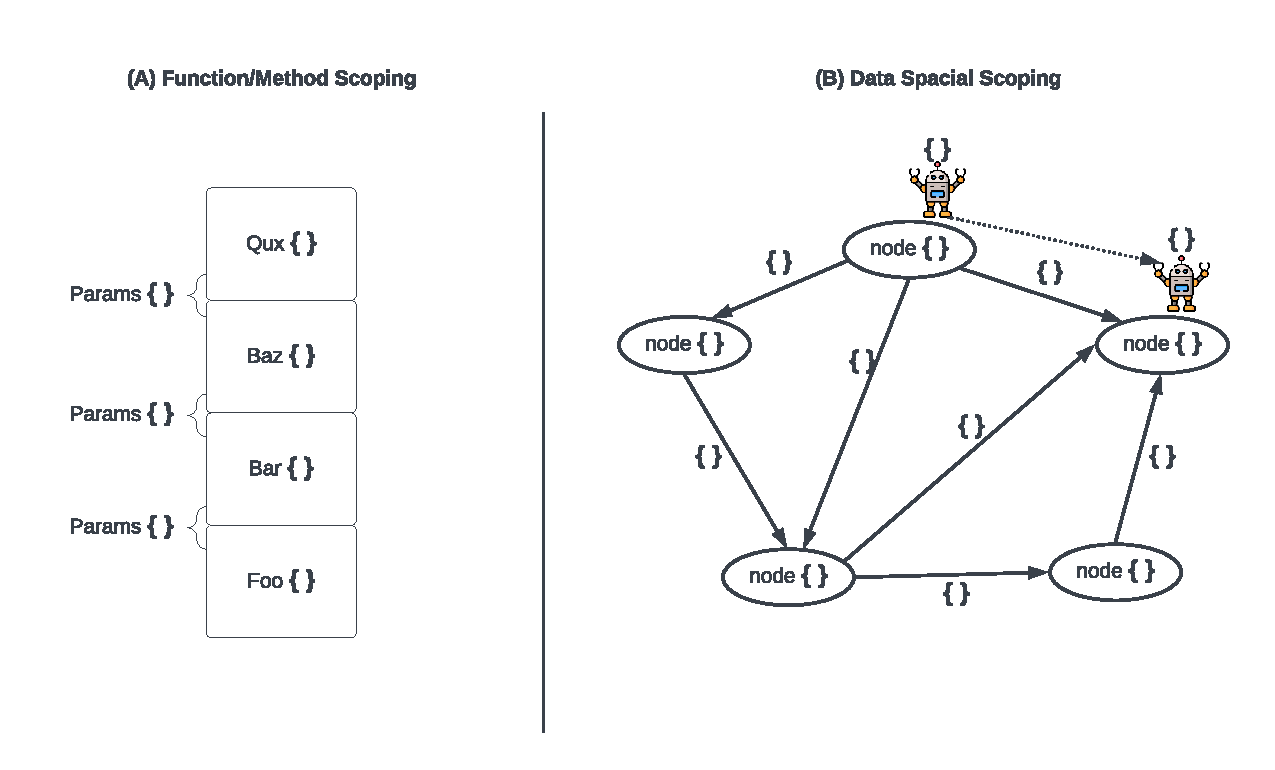
\includegraphics[width=\linewidth]{figures/data_spacial.pdf}
    \caption{A visualization of the behavior of scopes and problem solving abstractions provided by the near ubiquitous function / method based languages (left) and the data spacial programming model (right).}
    \label{fig:benefit}
\end{figure}

Traditionally in computer science, the task of raising the level abstraction in a computational model has primarily been for the goal of increasing programmer productivity.
This productivity comes from allowing engineers to function at the problem level while hiding the complexity of the underlying system.
The Jac language introduces a set of new abstractions guided by these principles based on two key insights.
First, Jac recognizes the emerging need for programmers to reason about and solve problems with graph representations of data.
Second, Jac further supports the need for algorithmic modularity and encapsulation to change and prototype production software in place of prior running codebases.
Based on these insights, we introduce two new sets of abstractions.
As shown in Figure~\ref{fig:benefit}b, Jac's \textbf{data-spacial scoping} natively facilitates graph based problem solving by replacing the traditional \emph{temporal} notion of scope with a function's activation record with scoping that is flattened and spatially laid out in graph structure.
This type of scoping allows for richer semantics for the organization of the data relevant to the problem being solved.
Figure~\ref{fig:benefit}b also depicts Jac's \textbf{agent oriented programming} as little robots.
Each robot carries scope with it as it walks and performs compute relevant to where it sits on the graph.
These `agent' abstractions capture the need for algorithmic modality and encapsulation when introducing solutions to already sophisticated codebases.
Jac can be used solely to build out complete solutions or as glue code with components built in other languages.
By leveraging these new language abstractions, HomeLendingPal~\cite{hlp-website} was able to create a production grade conversational AI experience with $\sim$300 lines of code in contrast to the tens of thousands it would take to build in a traditional programming language.
\section{A Novel Underlying Technology Stack}
\begin{figure}[tb]
    \centering
    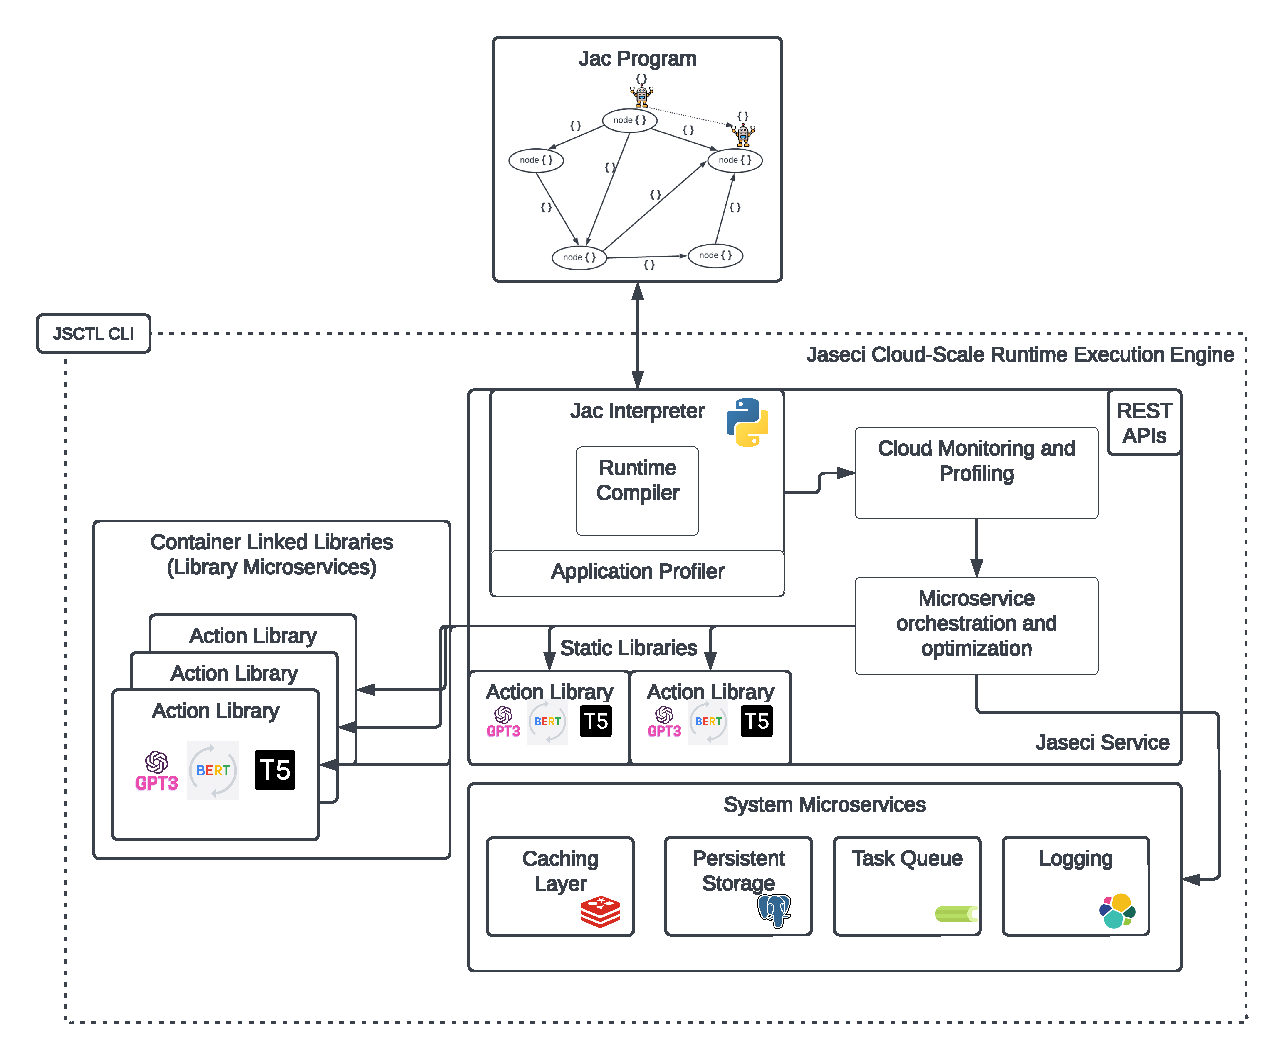
\includegraphics[width=\linewidth]{figures/jaseci_arch.pdf}
    \caption{The architecture of the Jaseci diffuse runtime execution. The runtime stack includes and combines information from interpreter level profiling, cloud monitoring and profiling, microservice orchestrator and optimizer. Container linked libraries are also depicted. }
    \label{fig:benefit2}
\end{figure}

Jaseci's cloud-scale runtime engine presents a higher level abstraction of the software stack.
The \emph{diffuse} runtime engine subsumes responsibility not only for the optimization of program code, but also the orchestration, configuration, and optimization of constituent micro services and the full cloud compute stack.
Duties such as container formation, microservice scaling, scheduling and optimization are automated by the runtime.
For example, as shown in Figure~\ref{fig:benefit2}c Jaseci introduces the concept of \textbf{container linked libraries} to complement traditional notions of statically and dynamically linked libraries.
From the programmers perspective, they need not know whether a call to a library is fused with the running programming instance or a remote call to a microservice somewhere in a cluster.
The decisioning of what \emph{should} be a microservice and what should be statically in the programs object scope is made automatically and seamlessly by the Jaseci \textbf{microservice orchestration engine}.
Underlying in-cluster microservices are encapsulated and hidden with this abstraction.
With the runtime having full visibility and control over the diffuse application, high complexity runtime decisions and heuristics such as autoscaling is brought under the purview of the runtime software stack, relieving the need of manual configuration.
With this Jaseci runtime, a single frontend engineer was able to implement the full ZeroShotBot~\cite{zsb-website} application (which uses a number of transformer neural networks) without writing a single line of traditional `backend' code.
This implementation currently support tens of thousands of queries a day across about $\sim$12 business customers with tens of thousands of individual end users in a single production environment.
\section{Battle Testing so Far...}

Jaseci is available on Github~\cite{jaseci-github} under MIT open source license and is composed of an ecosystem of tools spanning 3 packages.
These include \textbf{Jaseci Core}, its core execution engine,  \textbf{Jaseci Serv}, its diffuse runtime cloud-scale execution engine, and \textbf{Jaseci Kit}, a collection of cutting edge AI engines provided by the Jaseci community.
In addition to these main codebases, an experimental toolkit we call \textbf{Jaseci Studio} is in development to provide visual programming and debugging tooling for developers building with Jaseci.

There are a number of notable examples of Jaseci's use in production.
These users include  four selected start-up companies that have adopted Jac and Jaseci as their development engine and have already launched their products built using Jaseci.

\indent \textbf{ myca.ai}~\cite{myca-website} - a B2C personal productivity platform that uses AI to understand personal behavior trends and help users allocate their time, prioritize their tasks and achieve personal growth goals. Using Jaseci, myca.ai’s back-end development only took 1 month and myca.ai was launched within 3 months’ development to the public. Myca.ai is one of the fast growing personal growth tool and has received positive feedback from their users.

\indent \textbf{ZeroShotBot}~\cite{zsb-website} - a B2B company that develops a cutting edge conversational AI platform using Jaseci. The product development took 2 months and was done by frontend engineers. Zeroshotbot has gained significant market traction and has been in business discussions with major logos such as Volaris, Pizzahut to provide readily deployable FAQ chatbots.



\indent \textbf{Truselph}~\cite{ts-website} - A minority founded startup. Truselph creates an avatar of the person and builds conversational intelligence that allows the general public to interact with the avatar and ask questions, while the avatar will be able to provide personalized answers with emotions and facial expressions. Truselph is in partnership with Lenovo to co-develop Truselph powered Kiosks for retail stores and is in business discussions with chains such as Sephora.


\indent \textbf{ Home Lending Pal}~\cite{hlp-website} - an AI Powered Mortgage Advisor. Home Lending Pal is a minority founded start-up that helps people, especially under-served minority population to navigate through the mortgage and home purchase process. Home Lending Pal adopted Jaseci to provide two main product features: 1 - personalized mortgage advice and 2 - Kev, an AI-powered chatbot that will answer users questions about the process and give them a plan to improve their finances.
\section{In a Nutshell}
Jaseci is a novel computational model invented, designed and implemented to address this challenge.
Jaseci includes a novel programming model we call \emph{data-spacial programming} and a runtime engine we call the \emph{diffuse execution environment} to enable rapid development of large scale and nimble AI applications.
Our initial infrastructure has been used in practice to achieve 10x reduction in development time and near 100\% elimination of typical backend code needed for a complicated AI based application.
Jaseci~\cite{jaseci-website} was open sourced in 2021~\cite{jaseci-github}~\cite{jaseci-pypi}.
Today Jaseci is in production with 4 distinct commercial products built on the engine, including Myca~\cite{myca-website}, HomeLendingPal~\cite{hlp-website},  ZeroShotBot~\cite{zsb-website} and TrueSelph~\cite{ts-website}.




\chapter{Abstrations of Jaseci}
\minitoc
\section{Graphs, the Friend that Never Gets Invited to the Party}
There's something quite strange that has happend with our \gls{common languages} over the years, ...decades. When you look at it, almost every data structure we programmers use to solve problems can be modeled formally as a graph, or a special case of a graph, (save perhaps hash tables). Think about it, stacks, lists, queues, trees, heaps, and yes, even graphs, can be modeled with graphs. But, low and behold, no common language ustilizes the formal semantics of a graph as its first order abstraction for data or memory. I mean, isn't it a bit odd that practically every data structure covered in the language-agnostic classic foundational work \textit{Introduction to Algorithms}~\cite{intro_to_algo} can most naturally be be reasoned about as a graph, yet none of the common languages have built in and be designed around this primitive. I submit that the graph semantic is stupidly rich, very nice for us humans to reason about, and, most importantly for the purpose of Jaseci, is inherently well suited for the conceptualization and reasoning about computational problems, especially AI problems.
\par
There are a few arguments that may pop into mind at this point of my conjecture.
\begin{itemize}
    \item ``Well there are graph libraries in my favorite language that implement graph symantics, why would I need a language to force the concept upon me?''
          or
    \item ``Duh! Interacting with all data and memory through graphical abstractions will make the language ssllooowww as hell since memory in hardware is essitially a big array, what is this dude talking about!?!?''
\end{itemize}
\par
For the former of these two challenges, I counter with two points. First, the core design languages are always based upon their inherent abstractions. With graphs not being one such abstraction, the language's design will not be optimized to empower programmers to nimbly do gymnastics with rich language symantics that correspond to the rich semantics graphs offer (You'll see what I mean in later chapters).
\par
For the latter question, I'd respond, ``Have you SEEN the kind of abstractions in modern languages!?!? It's rediculous, lets look at python dictionaries, actually scratch that, lets keep it simple and look at dynamic typing in general. The runtime complexity to support dynamic typing is most certainly higher than what would be needed to support graph symantics. Duh right back at'ya!''
\subsection{Yes, But What Kind of Graphs}

There are many categories of graphs to consider when thinking about the abstractions to support in Jaseci. There are rules to be defined as to the availabe semantics of the graphs. Should all graphs be \gls{directed graphs}, should we allow the creation of \gls{undirected graphs}, what about parallel edges or \gls{multigraphs}, are those explicitly expressible or discouraged / banned, can we express \gls{hypergraphs}, and what combination of these graphical sematics should be able to be manifested and manipulated through the programming model. At this point I can feel your eyes getting droopy and your mind moving into that intermediary state between concious and sleeping, so let me cut to the answer.
\par
\printfigGraphTypes
In Jaseci, we elect to assume the following semantics:
\begin{enumerate}
    \item Graphs are directed (as per Figure~\ref{fig:directedgraph}) with a special case of a doubly directed edge type which can be utilized practically as an undirected edge (imagine fusing the two edges between nodes 3 and 4 in the figure).
    \item Both nodes and edges have their own distinct identities (i,e. an edge isn't representable as a pairing of two nodes). This point is important as both nodes and edges can have \gls{contexts}.
    \item Multigraphs (i.e., parallel edges) are allowed, including self-loop edges (as per Figure~\ref{fig:multigraph}).
    \item Graphs are not required to be acyclic.
    \item No hypergraphs, as I wouldn't want Jaseci programmers heads to explode.

\end{enumerate}
\emph{As an aside, I would describe Jaseci graphs as strictly unstrict directed multigraphs that leverages the semantics of parallel edges to create a laymans `undirected edge' by shorthanding two directed edges pointed in opposite directions between the same two nodes.}
\par
\begin{nerd}
    I'd formally describe a Jaseci Graph as an $7$-tuple $(N,E,C,s,t,c_N,c_E)$, where
    \begin{enumerate}
        \item $N$ is the set of nodes in a graph
        \item $E$ is the set of edges in a graph
        \item $C$ is the set of all contexts
        \item $s$: $E \rightarrow V$, maps the source node to an edge
        \item $t$: $E \rightarrow V$,  maps the target node to an edge
        \item $c_N$: $N \rightarrow C$, maps nodes to contexts
        \item $c_E$: $E \rightarrow C$, maps edges to contexts
    \end{enumerate}
    An undriected edge can then be formed with a pair of edges $(x, y)$ if three conditions are met,
    \begin{enumerate}
        \item $x, y \in E$
        \item $s(x) = t(y)$, and $s(y) = t(x)$
        \item $c_E(x) = c_E(y)$
    \end{enumerate}
\end{nerd}
\par
If you happend to have read that formal definition and didn't enter deep comatose you may be wondering ``Whoa, what was that context stuff that came outta nowhere! What's this guy trying to do here, sneaking a new concept in as if it was already introduced and described.''
\par
Worry not friend, lets discuss.
\subsection{Putting it All Into Context}

A key principle of Jaseci is to reshape and reimagine how we view data and memory. We do so by fusing the concept of data with the intuitive and rich semantics of graphs as the lowest level primitive to view memory.

\begin{nerd}
    A context is a representation of data that can be expressed simply as a $3$-tuple $(\sum_K,\sum_V,p_K)$, where
    \begin{enumerate}
        \item $\sum_K$ is a finite alphabet of keys
        \item $\sum_V$ is a finite alphabet of values
        \item $p_K$ is the pairing of keys to values
    \end{enumerate}
\end{nerd}
\section{Walkers}
\section{Abilities}
\section{Actions}
\section{Other Abstractions Not Yet Actualized in Current Jaseci}


\chapter{Architecture of Jaseci and Jac}
\minitoc
\section{Anatomy of a Jaseci Application}
\section{The Jaseci Machine}
\subsection{Machine Core}
\subsection{Jaseci Cloud Server}

\chapter{Interfacing a Jaseci Machine}
\minitoc
\jacdot{dia_api_server_client}{.6}{Jaseci Interface Architecture}
Now that we know what Jaseci is all about, next lets roll up our sleeves and jump in. One of the best ways to jump into Jaseci world is to gather some sample Jac programs and start tinkering with them.
\par
Before we jump right into it, it's important to have a bit of an understanding of the the way the interface itself is architected from in the implementation of the Jaseci stack. Jaseci has a module that serves as its  the core interface (summarized in Table~\ref{tab:jsAPI}) to the Jaseci machine. This interface is expressed as a set of method functions within a python class in Jaseci  called \texttt{master}. (By the way, don't worry, it's ok to use ``master'', its not racialist, see Rant~\ref{rant:racistmaster} for more context). The `client' expressions of that interface in the forms of a command line tool \texttt{jsctl} and a server-side REST API built using Django~\footnote{Django ~\cite{django} is a Python web framework for rapid development and clean, pragmatic design}. Figure~\ref{dot:dia_api_server_client} illustrates this architecture representing the relationship between core APIs and client side expressions.

If I may say so myself the code architecture of interface generation from function signatures is elegant, sexy, and takes advantage of the best python has to offer in terms of its support for introspection. With this approach, as the set of functions and their semantics change in the \texttt{master} API class, both the JSCTL Cli tool and the REST Server-side API changes. We dig into this and tons more in the Part~\ref{part:crafting}, so we'll leave the discussion on implementation architecture there for the moment. Lets jump right into how we get started playing with some \gls{leet} Jaseci \gls{haxor}ing. First we start with JSCTL then dive into the REST API.


\section{JSCTL: The Jaseci Command Line Interface}
JSCTL or \texttt{jsctl} is a command line tool that provides full access to Jaseci. This tool is installed alongside the installation of the Jaseci Core package and should be accessible from the command line from anywhere. Let's say you've just checked out the Jaseci repo and you're in head folder. You should be able to execute the following.
\par
\shellout{jsctl_setup.shell}
\par
Here we've installed the Jaseci python package that can be imported into any python project with a directive such as \texttt{import jaseci}, and at the same time, we've installed the \texttt{jsctl} command line tool into our OS environment. At this point we can issue a call to say \texttt{jsctl --help} for any working directory.
\begin{nerd}
    Python Code~\ref{py:setup.py} shows the implementation of \texttt{setup.py} that is responsible for deploying the jsctl tool upon \texttt{pip3} installation of Jaseci Core.
    \pycode{setup.py}{setup.py for Jaseci Core}
\end{nerd}

\subsection{The Very Basics: CLI vs Shell-mode, and Session Files }
This command line tool provides full access to the Jaseci core APIs via the command line, or a shell mode. In shell mode, all of the same Jaseci API functionally is available within a single session. To invoke shell-mode, simply execute \texttt{jsctl} without any commands and jsctl will enter shell mode as per the example below.
\par
\shellout{jsctl_shell_mode.shell}
\par
Here we launched \texttt{jsctl} directly into shell mode for a single session and we can issue various calls to the Jaseci API for that session. In this example we issue a single call to \texttt{graph create}, which creates a graph within the Jaseci session with a single root node, then exit the shell with \texttt{exit}.
\par
The exact behavior can be achieved without ever entering the shell directly from the command line as shown below.
\par
\shellout{jsctl_cli_mode.shell}
\par
All such calls to Jaseci's API (summarized in Table~\ref{tab:jsAPI}) can be issued either through shell-mode and CLI mode.
\paragraph{Session Files}
At this point, it's important to understand how sessions work. In a nutshell, a session captures the complete state of a jaseci machine. This state includes the status of memory, graphs, walkers, configurations, etc. The complete state of a Jaseci machine can be captured in a \texttt{.session} file. Every time state changes for a given session via the \texttt{jsctl} tool the assigned session file is updated. If you've been following along so far, try this.
\par
\shellout{session_default.shell}
\par
Note from the first call to \texttt{ls} we have a session file that has been created call \texttt{js.session}. This is the default session file \texttt{jsctl} creates and utilizes when called either in cli mode or shell mode. After listing session files, notices the call to \texttt{graph list} which lists the root nodes of all graphs created within a Jaseci machine's state. Note \texttt{jsctl} lists two such graph root nodes. Indeed these nodes correspond to the ones we've just created when contrasting cli mode and shell mode above. Having these two graphs demonstrates that across both instantiations of \texttt{jsctl} the same session, \texttt{js.session}, is being used. Now try the following.
\par
\shellout{new_session.shell}
\par
Here we see that we can use the \texttt{-f} or \texttt{--filename} flag to specify the session file to use. In this case we list the graphs of the session corresponding to \texttt{mynew.session} and see the JSON representation of an empty list of objects. We then list session files and see that one was created for \texttt{mynew.session}. If we were to now type \texttt{jsctl --filename js.session graph list}, we would see a list of the two graph objects that we created earlier.
\paragraph{In-memory mode}
Its important to note that there is also an in-memory mode that can be created buy using the \texttt{-m} or \texttt{--mem-only} flags. This flag is particularly useful when you'd simply like to tinker around with a machine in shell-mode or you'd like to script some behavior to be executed in Jac and have no need to maintain machine state after completion. We will be using in memory session mode quite a bit, so you'll get a sense of its usage throughout this chapter. Next we actually see a workflow for tinkering.

\subsection{A Simple Workflow for Tinkering}

As you get to know Jaseci and Jac, you'll want to try things and tinker a bit. In this section, we'll get to know how \texttt{jsctl} can be used as the main platform for this play. A typical flow will involve jumping into shell-mode, writing some code, running that code to observe output, and in visualizing the state of the graph, and rendering that graph in dot to see it's visualization.
\paragraph{Install Graphvis}
Before we jump right in, let me strongly encourage you install Graphviz. Graphviz is open source graph visualization software package that includes a handy dandy command line tool call \texttt{dot}. Dot is also a standardized and open graph description language that is a key primitive of Graphviz. The \texttt{dot} tool in Graphviz takes dot code and renders it nicely. Graphviz is super easy to install. In Ubuntu simply type \texttt{sudo apt install graphviz}, or on mac type \texttt{brew install graphviz} and you're done! You should be able to call \texttt{dot} from the command line.
\par
Ok, lets start with a scenario. Say you'd like to write your first Jac program which will include some nodes, edges, and walkers and you'd like to print to standard output and see what the graph looks like after you run an interesting walker. Let role play.
\par
Lets hop into a \texttt{jsctl} shell.
\par
\shellout{wf_init.shell}
\par
Good, we're in! And we've set the session to be an in-memory session so no session file will be created or saved. For this play session we only care about the Jac program we write, which will be saved. The state of the Jaseci machine we run our toy program on doesn't really matter to us.
\par
Now that we've got our shell running, we first want to create a blank graph. Remember, all walkers, Jaseci's primary unit of computation, must run on a node. As default, we can use the root node of a freshly created graph, hence we need to create a base graph. But oh no! We're a bit rusty and have forgotten how create our initial graph using \texttt{jsctl}. Let's navigate the help menu to jog our memories.
\par
\shellout{wf_help_nav.shell}
\par
Ohhh yeah! That's it. After simply using \texttt{help} from the shell we were able to navigate to the relevant info for \texttt{graph create}. Let's use this newly gotten wisdom.
\par
\shellout{wf_graph.shell}
\par
Great! With this command a graph is created and a single root node is born. \texttt{jsctl} shares with us the details of this root graph node. In Jaseci, graphs are referenced by their root nodes and every graph has a single root node.
\par
Notice we've also set the \texttt{-set\_active} parameter to true. This parameter informs Jaseci to use the root node of this graph (in particular the UUID of this root node) as the default parameter to all future calls to Jaseci Core APIs that have a parameter specifying a graph or node to operate on. This global designation that this graph is the `active' graph is a convenience feature so we the user doesn't have to specify this parameter for future calls. Of course this can be overridden, more on that later.
\par
Next, lets write some Jac code for our little program. \texttt{jsctl} has a built in editor that is simple yet powerful. You can use either this built in editor, or your favorite editor to create the \texttt{.jac} file for our toy program. Let's use the built in editor.
\par
\shellout{wf_edit_jac.shell}
\par
The \texttt{edit} command invokes the built in editor. Though it's a terminal editor based on \texttt{ncurses}, you can basically use it much like you'd use any wysiwyg editor with features like standard cut \texttt{ctrl-c} and paste \texttt{ctrl-v}, mouse text selection, etc. It's based on the phenomenal pure python project from Google called \texttt{ci\_edit}. For more detailed help cheat sheet see Appendix. If you must use your own favorite editor, simply be sure that you save the fam.jac file in the same working directory from which you are running the Jaseci shell. Now type out the toy program in Jac Code~\ref{jac:fam.jac}.
\par
\jaccode{fam.jac}{Jac Family Toy Program}
\par
Don't worry if that looks like the most cryptic \gls{gobbledygook} you've ever seen in your life. As you learn the Jac language, all will become clear. For now, lets tinker around. Now save and quit the editor. If you are using the built in editor thats simply a \texttt{ctrl-s, ctrl-q} combo.
\par
Ok, now we should have a \texttt{fam.jac} file saved in our working directory. We can check from the Jaseci shell!
\par
\shellout{wf_ls.shell}
\par
We can list files from the shell prompt. By default the \texttt{ls} command only lists files relevant to Jaseci (i.e., \texttt{*.jac}, \texttt{*.dot}, etc). To list all files simply add a \texttt{--all} or \texttt{-a}.
\par
Now, on to what is on of the key operations. Lets ``register'' a \gls{sentinel} based on our Jac program. A sentinel is the abstraction Jaseci uses to encapsulate compiled walkers and architype nodes and edges. You can think of registering a sentinel as compiling your jac program. The walkers of a given sentinel can then be invoked and run on arbitrary nodes of any graph. Let's register our Jac toy program.
\par
\shellout{wf_sent_reg.shell}
\par
Ok, theres a lot that just happened there. First, we see some logging output that informs us that the Jac code is being processed (which really means the Jac program is being parsed and IR being generated). If there are any syntax errors or other issues, this is where the error output will be printed along with any problematic lines of code and such. If all goes well, we see the next logging output that the code has been successfully registered. The formal output is the relevant details of the successfully created sentinel. Note, that we've also made this the ``active'' sentinel meaning it will be used as the default setting for any calls to Jaseci Core APIs that require a sentinel be specified. At this point, Jaseci has registered our code and we are ready to run walkers!
\par
But first, lets take a quick look at some of the objects loaded into our Jaseci machine. For this I'll briefly introduce the \texttt{alias} group of APIs.
\par
\shellout{wf_aliases.shell}
\par
The \texttt{alias} set of APIs are designed as an additional set of convenience tools to simplify the referencing of various objects (walkers, architypes, etc) in Jaseci. Instead of having to use the UUIDs to reference each object, an alias can be used to refer to any object. These aliases can be created or removed utilizing the \texttt{alias} APIs.
\par
Upon registering a sentinel, a set of aliases are automatically created for each object produced from processing the corresponding Jac program. The call to \texttt{alias list} lists all available aliases in the session. Here, we're using this call to see the objects that were created for our toy program and validate it corresponds to the ones we would expect from the Jac Program represented in JC~\ref{jac:fam.jac}. Everything looks good!
\par
Now, for the big moment! lets run our walker on the root node of the graph we created and see what happens!
\par
\shellout{wf_run_walker.shell}
\par
Sweet!! We see the standard output we'd expect from our toy program. Hrm, as we'd expect, when it comes to the family, the man doesn't do much it seems.
\par
But there were many semantics to what our toy program does. How do we visualize that the graph produced by or program is right. Well we're in luck! We can use Jaseci `dot' features to take a look at our graph!!
\par
\shellout{wf_dot_render.shell}
\par
\jacdot{fam}{.3}{Graph for \texttt{fam.jac}}
Here we've used the \texttt{graph get} core API to get a print out of the graph in dot format. By default \texttt{graph get} dumps out a list of all edge and node objects of the graph, however with the \texttt{-mode dot} parameter we've specified that the graph should be printed in dot. The \texttt{-o} flag specifies a file to dump the output of the command. Note that the \texttt{-o} flag for \texttt{jsctl} commands only outputs the formal returned data (json payload, or string) from a Jaseci Core API. Logging output, standard output, etc will not be saved to the file though anything reported by a walker using \texttt{report} will be saved. This output file directive is \texttt{jsctl} specific and work with any command given to \texttt{jsctl}.
\par
To see a pretty visual of the graph itself, we can use the \texttt{dot} command from Graphviz. Simply type \texttt{dot -Tpdf fam.dot -o fam.pdf} and Voila! We can see the beautiful graph our toy Jac program has produced on its way to the standard output.
\par
Awesomeness! We are Jac \Gls{haxor}s now!

\section{Jaseci REST API}
\subsection{API Parameter Cheatsheet}
\printtabJSAPI
\section{Full Spec of Jaseci Core APIs}
\subsection{APIs for actions}

\par
This set action APIs enable the manual management of Jaseci actions and action
libraries/sets. Action libraries can be loaded locally into the running instance of
the python program, or as a remote container linked action library. In this mode,
action libraries operate as micro-services. Jaseci will be able to dynamically
and automatically make this decision for the user based on online monitoring and
performance profiling.

\subsubsection{\lstinline[basicstyle=\Large\ttfamily]$actions load local$}

\apispec{cli: actions load local | api: actions\_load\_local | auth: admin}{file: str (*req)}
{This API will dynamically load a module based on a python file. The module
is loaded directly into the running Jaseci python instance. This API also
makes an attempt to auto detect and hot load any python package dependencies
the file may reference via python's relative imports. This file is assumed to
have the necessary annotations and decorations required by Jaseci to recognize
its actions.\vspace{4mm}\par
\argspec{Parameters}{
\texttt{file} -- The python file with full to load actions from.
(i.e., ~/local/myact.py)\vspace{1.5mm}\par
}}
\subsubsection{\lstinline[basicstyle=\Large\ttfamily]$actions load remote$}

\apispec{cli: actions load remote | api: actions\_load\_remote | auth: admin}{url: str (*req)}
{This API will dynamically load a set of actions that are present on a remote
server/micro-service. This server must be configured to interact with Jaseci
properly. This is easily achieved using the same decorators used for local
action libraries. Remote actions allow for higher flexibility in the languages
supported for action libraries. If an  library writer would like to use another
language, the main hook REST api simply needs to be implemented. Please
refer to documentation on creating action libraries for more details.\vspace{4mm}\par
\argspec{Parameters}{
\texttt{url} -- The url of the API server supporting Jaseci actions.\vspace{1.5mm}\par
}}
\subsubsection{\lstinline[basicstyle=\Large\ttfamily]$actions load module$}

\apispec{cli: actions load module | api: actions\_load\_module | auth: admin}{mod: str (*req)}
{This API will dynamically load a module using python's module import format.
This is particularly useful for pip installed action libraries as the developer
can directly reference the module using the same format as a regular python
import. As with load local, the module will be loaded directly into the running
Jaseci python instance.\vspace{4mm}\par
\argspec{Parameters}{
\texttt{mod} -- The import style module to load actions from.
(i.e., jaseci\_kit.bi\_enc)\vspace{1.5mm}\par
}}
\subsubsection{\lstinline[basicstyle=\Large\ttfamily]$actions list$}

\apispec{cli: actions list | api: actions\_list | auth: admin}{name: str ()}
{This API is used to list the loaded actions active in Jaseci. These actions
include all types of loaded actions whether it be local modules or remote
containers. A particular set of actions can be viewed using the name parameter.\vspace{4mm}\par
\argspec{Parameters}{
\texttt{name} -- The name for a library for which to filter the view of shown
actions. If left blank all actions from all loaded sets will be shown.\vspace{1.5mm}\par
}}
\subsection{APIs for alias}

\par
The alias set of APIs provide a set of `alias' management functions for
creating and managing aliases for long strings such as UUIDs. If an alias'
name is used as a parameter value in any API call, that parameter will see
the alias' value instead. Given that references to all sentinels, walkers,
nodes, etc. utilize UUIDs, it becomes quite useful to create pneumonic
names for them. Also, when registering   sentinels, walkers, architype
handy aliases are automatically generated. These generated aliases can
then be managed using the alias APIs. Keep in mind that whenever an alias
is created, all parameter values submitted to any API with the alias name
will be replaced internally by its value. If you get in a bind, simply use
the clear or delete alias APIs.

\subsubsection{\lstinline[basicstyle=\Large\ttfamily]$alias register$}

\apispec{cli: alias register | api: alias\_register | auth: user}{name: str (*req), value: str (*req)}
{Either create new alias string to string mappings or replace
an existing mappings of a given alias name. Once registered the
alias mapping is instantly active.\vspace{4mm}\par
\argspec{Parameters}{
\texttt{name} -- The name for the alias created by caller.\vspace{1.5mm}\par

\texttt{value} -- The value for that name to map to (i.e., UUID)\vspace{1.5mm}\par
}\vspace{4mm}\par
\argspec{Returns}{Fields include
'response': Message of mapping that was created}}
\subsubsection{\lstinline[basicstyle=\Large\ttfamily]$alias list$}

\apispec{cli: alias list | api: alias\_list | auth: user}{n/a}
{Returns dictionary object of name to value mappings currently active.
This API is quite useful to track not only the aliases the caller
creates, but also the aliases automatically created as various Jaseci
objects (walkers, architypes, sentinels, etc.) are created, changed,
or destroyed.\vspace{4mm}\par
\argspec{Returns}{Dictionary of active mappings
'name': 'value'
...}}
\subsubsection{\lstinline[basicstyle=\Large\ttfamily]$alias delete$}

\apispec{cli: alias delete | api: alias\_delete | auth: user}{name: str (*req)}
{Removes a specific alias by its name. Only the alias is removed no
actual objects are affected. Future uses of this name will not be
mapped.\vspace{4mm}\par
\argspec{Parameters}{
\texttt{name} -- The name for the alias to be removed from caller.\vspace{1.5mm}\par
}\vspace{4mm}\par
\argspec{Returns}{Fields include
'response': Message of success/failure to remove alias
'success': True/False based on delete actually happening}}
\subsubsection{\lstinline[basicstyle=\Large\ttfamily]$alias clear$}

\apispec{cli: alias clear | api: alias\_clear | auth: user}{n/a}
{Removes a all aliases. No actual objects are affected. Aliases will
continue to be automatically generated when creating other Jaseci
objects.\vspace{4mm}\par
\argspec{Returns}{Fields include
'response': Message of number of alias removed
'removed': Number of aliases removed}}
\subsection{APIs for architype}

\par
The architype set of APIs allow for the addition and removing of
architypes. Given a Jac implementation of an architype these APIs are
designed for creating, compiling, and managing architypes that can be
used by Jaseci. There are two ways to add an architype to Jaseci, either
through the management of sentinels using the sentinel API, or by
registering independent architypes with these architype APIs. These
APIs are also used for inspecting and managing existing arichtypes that
a Jaseci instance is aware of.

\subsubsection{\lstinline[basicstyle=\Large\ttfamily]$architype register$}

\apispec{cli: architype register | api: architype\_register | auth: user}{code: str (*req), encoded: bool (False), snt: sentinel (None)}
{This register API allows for the creation or replacement/update of
an architype that can then be used by walkers in their interactions
of graphs. The code argument takes Jac source code for the single
architype. To load multiple architypes and walkers at the same time,
use sentinel register API.\vspace{4mm}\par
\argspec{Parameters}{
\texttt{code} -- The text (or filename) for an architypes Jac code\vspace{1.5mm}\par

\texttt{encoded} -- True/False flag as to whether code is encode
in base64\vspace{1.5mm}\par

\texttt{snt} -- The UUID of the sentinel to be the owner of this
architype\vspace{1.5mm}\par
}\vspace{4mm}\par
\argspec{Returns}{Fields include
'architype': Architype object if created otherwise null
'success': True/False whether register was successful
'errors': List of errors if register failed
'response': Message on outcome of register call}}
\subsubsection{\lstinline[basicstyle=\Large\ttfamily]$architype get$}

\apispec{cli: architype get | api: architype\_get | auth: user}{arch: architype (*req), mode: str (default), detailed: bool (False)}
{No documentation yet.\vspace{4mm}\par
\argspec{Parameters}{
\texttt{arch} -- The architype being accessed\vspace{1.5mm}\par

\texttt{mode} -- Valid modes: {default, code, ir, }\vspace{1.5mm}\par

\texttt{detailed} -- Flag to give summary or complete set of fields\vspace{1.5mm}\par
}\vspace{4mm}\par
\argspec{Returns}{Fields include (depends on mode)
'code': Formal source code for architype
'ir': Intermediate representation of architype
'architype': Architype object print}}
\subsubsection{\lstinline[basicstyle=\Large\ttfamily]$architype set$}

\apispec{cli: architype set | api: architype\_set | auth: user}{arch: architype (*req), code: str (*req), mode: str (default)}
{No documentation yet.\vspace{4mm}\par
\argspec{Parameters}{
\texttt{arch} -- The architype being set\vspace{1.5mm}\par

\texttt{code} -- The text (or filename) for an architypes Jac code/ir\vspace{1.5mm}\par

\texttt{mode} -- Valid modes: {default, code, ir, }\vspace{1.5mm}\par
}\vspace{4mm}\par
\argspec{Returns}{Fields include (depends on mode)
'success': True/False whether set was successful
'errors': List of errors if set failed
'response': Message on outcome of set call}}
\subsubsection{\lstinline[basicstyle=\Large\ttfamily]$architype list$}

\apispec{cli: architype list | api: architype\_list | auth: user}{snt: sentinel (None), detailed: bool (False)}
{No documentation yet.\vspace{4mm}\par
\argspec{Parameters}{
\texttt{snt} -- The sentinel for which to list its architypes\vspace{1.5mm}\par

\texttt{detailed} -- Flag to give summary or complete set of fields\vspace{1.5mm}\par
}\vspace{4mm}\par
\argspec{Returns}{List of architype objects}}
\subsubsection{\lstinline[basicstyle=\Large\ttfamily]$architype delete$}

\apispec{cli: architype delete | api: architype\_delete | auth: user}{arch: architype (*req), snt: sentinel (None)}
{No documentation yet.\vspace{4mm}\par
\argspec{Parameters}{
\texttt{arch} -- The architype being set\vspace{1.5mm}\par

\texttt{snt} -- The sentinel for which to list its architypes\vspace{1.5mm}\par
}\vspace{4mm}\par
\argspec{Returns}{Fields include (depends on mode)
'success': True/False whether command was successful
'response': Message on outcome of command}}
\subsection{APIs for config}

Abstracted since there are no valid configs in core atm, see jaseci\_serv
to see how used.

\subsubsection{\lstinline[basicstyle=\Large\ttfamily]$config get$}

\apispec{cli: config get | api: config\_get | auth: admin}{name: str (*req), do_check: bool (True)}
{No documentation yet.}
\subsubsection{\lstinline[basicstyle=\Large\ttfamily]$config set$}

\apispec{cli: config set | api: config\_set | auth: admin}{name: str (*req), value: str (*req), do_check: bool (True)}
{No documentation yet.}
\subsubsection{\lstinline[basicstyle=\Large\ttfamily]$config list$}

\apispec{cli: config list | api: config\_list | auth: admin}{n/a}
{No documentation yet.}
\subsubsection{\lstinline[basicstyle=\Large\ttfamily]$config index$}

\apispec{cli: config index | api: config\_index | auth: admin}{n/a}
{No documentation yet.}
\subsubsection{\lstinline[basicstyle=\Large\ttfamily]$config exists$}

\apispec{cli: config exists | api: config\_exists | auth: admin}{name: str (*req)}
{No documentation yet.}
\subsubsection{\lstinline[basicstyle=\Large\ttfamily]$config delete$}

\apispec{cli: config delete | api: config\_delete | auth: admin}{name: str (*req), do_check: bool (True)}
{No documentation yet.}
\subsection{APIs for global}

No documentation yet.

\subsubsection{\lstinline[basicstyle=\Large\ttfamily]$global set$}

\apispec{cli: global set | api: global\_set | auth: admin}{name: str (*req), value: str (*req)}
{No documentation yet.}
\subsubsection{\lstinline[basicstyle=\Large\ttfamily]$global delete$}

\apispec{cli: global delete | api: global\_delete | auth: admin}{name: str (*req)}
{No documentation yet.}
\subsubsection{\lstinline[basicstyle=\Large\ttfamily]$global sentinel set$}

\apispec{cli: global sentinel set | api: global\_sentinel\_set | auth: admin}{snt: sentinel (None)}
{No documentation yet.}
\subsubsection{\lstinline[basicstyle=\Large\ttfamily]$global sentinel unset$}

\apispec{cli: global sentinel unset | api: global\_sentinel\_unset | auth: admin}{n/a}
{No documentation yet.}
\subsection{APIs for graph}

No documentation yet.

\subsubsection{\lstinline[basicstyle=\Large\ttfamily]$graph create$}

\apispec{cli: graph create | api: graph\_create | auth: user}{set_active: bool (True)}
{No documentation yet.}
\subsubsection{\lstinline[basicstyle=\Large\ttfamily]$graph get$}

\apispec{cli: graph get | api: graph\_get | auth: user}{gph: graph (None), mode: str (default), detailed: bool (False)}
{Valid modes: {default, dot, }}
\subsubsection{\lstinline[basicstyle=\Large\ttfamily]$graph list$}

\apispec{cli: graph list | api: graph\_list | auth: user}{detailed: bool (False)}
{No documentation yet.}
\subsubsection{\lstinline[basicstyle=\Large\ttfamily]$graph active set$}

\apispec{cli: graph active set | api: graph\_active\_set | auth: user}{gph: graph (*req)}
{No documentation yet.}
\subsubsection{\lstinline[basicstyle=\Large\ttfamily]$graph active unset$}

\apispec{cli: graph active unset | api: graph\_active\_unset | auth: user}{n/a}
{No documentation yet.}
\subsubsection{\lstinline[basicstyle=\Large\ttfamily]$graph active get$}

\apispec{cli: graph active get | api: graph\_active\_get | auth: user}{detailed: bool (False)}
{No documentation yet.}
\subsubsection{\lstinline[basicstyle=\Large\ttfamily]$graph delete$}

\apispec{cli: graph delete | api: graph\_delete | auth: user}{gph: graph (*req)}
{No documentation yet.}
\subsubsection{\lstinline[basicstyle=\Large\ttfamily]$graph node get$}

\apispec{cli: graph node get | api: graph\_node\_get | auth: user}{nd: node (*req), keys: list ([])}
{No documentation yet.}
\subsubsection{\lstinline[basicstyle=\Large\ttfamily]$graph node set$}

\apispec{cli: graph node set | api: graph\_node\_set | auth: user}{nd: node (*req), ctx: dict (*req), snt: sentinel (None)}
{No documentation yet.}
\subsubsection{\lstinline[basicstyle=\Large\ttfamily]$graph walk$}

\apispec{cli: graph walk (cli only)}{nd: node (None)}
{No documentation yet.}
\subsection{APIs for jac}

No documentation yet.

\subsubsection{\lstinline[basicstyle=\Large\ttfamily]$jac build$}

\apispec{cli: jac build (cli only)}{file: str (*req), out: str ()}
{No documentation yet.}
\subsubsection{\lstinline[basicstyle=\Large\ttfamily]$jac test$}

\apispec{cli: jac test (cli only)}{file: str (*req), detailed: bool (False)}
{and .jir executables}
\subsubsection{\lstinline[basicstyle=\Large\ttfamily]$jac run$}

\apispec{cli: jac run (cli only)}{file: str (*req), walk: str (init), ctx: dict (\{\}), profiling: bool (False)}
{and .jir executables}
\subsubsection{\lstinline[basicstyle=\Large\ttfamily]$jac dot$}

\apispec{cli: jac dot (cli only)}{file: str (*req), walk: str (init), ctx: dict (\{\}), detailed: bool (False)}
{files and .jir executables}
\subsection{APIs for logger}

No documentation yet.

\subsubsection{\lstinline[basicstyle=\Large\ttfamily]$logger http connect$}

\apispec{cli: logger http connect | api: logger\_http\_connect | auth: admin}{host: str (*req), port: int (*req), url: str (*req), log: str (all)}
{Valid log params: {sys, app, all }}
\subsubsection{\lstinline[basicstyle=\Large\ttfamily]$logger http clear$}

\apispec{cli: logger http clear | api: logger\_http\_clear | auth: admin}{log: str (all)}
{Valid log params: {sys, app, all }}
\subsubsection{\lstinline[basicstyle=\Large\ttfamily]$logger list$}

\apispec{cli: logger list | api: logger\_list | auth: admin}{n/a}
{No documentation yet.}
\subsection{APIs for master}

\par
These APIs

\subsubsection{\lstinline[basicstyle=\Large\ttfamily]$master create$}

\apispec{cli: master create | api: master\_create | auth: user}{name: str (*req), global_init: str (), global_init_ctx: dict (\{\}), other_fields: dict (\{\})}
{other fields used for additional feilds for overloaded interfaces
(i.e., Dango interface)}
\subsubsection{\lstinline[basicstyle=\Large\ttfamily]$master get$}

\apispec{cli: master get | api: master\_get | auth: user}{name: str (*req), mode: str (default), detailed: bool (False)}
{Valid modes: {default, }}
\subsubsection{\lstinline[basicstyle=\Large\ttfamily]$master list$}

\apispec{cli: master list | api: master\_list | auth: user}{detailed: bool (False)}
{No documentation yet.}
\subsubsection{\lstinline[basicstyle=\Large\ttfamily]$master active set$}

\apispec{cli: master active set | api: master\_active\_set | auth: user}{name: str (*req)}
{NOTE: Specail handler included in general interface to api}
\subsubsection{\lstinline[basicstyle=\Large\ttfamily]$master active unset$}

\apispec{cli: master active unset | api: master\_active\_unset | auth: user}{n/a}
{No documentation yet.}
\subsubsection{\lstinline[basicstyle=\Large\ttfamily]$master active get$}

\apispec{cli: master active get | api: master\_active\_get | auth: user}{detailed: bool (False)}
{No documentation yet.}
\subsubsection{\lstinline[basicstyle=\Large\ttfamily]$master self$}

\apispec{cli: master self | api: master\_self | auth: user}{detailed: bool (False)}
{No documentation yet.}
\subsubsection{\lstinline[basicstyle=\Large\ttfamily]$master delete$}

\apispec{cli: master delete | api: master\_delete | auth: user}{name: str (*req)}
{No documentation yet.}
\subsection{APIs for object}

\par
...

\subsubsection{\lstinline[basicstyle=\Large\ttfamily]$global get$}

\apispec{cli: global get | api: global\_get | auth: user}{name: str (*req)}
{No documentation yet.}
\subsubsection{\lstinline[basicstyle=\Large\ttfamily]$object get$}

\apispec{cli: object get | api: object\_get | auth: user}{obj: element (*req), depth: int (0), detailed: bool (False)}
{No documentation yet.}
\subsubsection{\lstinline[basicstyle=\Large\ttfamily]$object perms get$}

\apispec{cli: object perms get | api: object\_perms\_get | auth: user}{obj: element (*req)}
{No documentation yet.}
\subsubsection{\lstinline[basicstyle=\Large\ttfamily]$object perms set$}

\apispec{cli: object perms set | api: object\_perms\_set | auth: user}{obj: element (*req), mode: str (*req)}
{No documentation yet.}
\subsubsection{\lstinline[basicstyle=\Large\ttfamily]$object perms default$}

\apispec{cli: object perms default | api: object\_perms\_default | auth: user}{mode: str (*req)}
{No documentation yet.}
\subsubsection{\lstinline[basicstyle=\Large\ttfamily]$object perms grant$}

\apispec{cli: object perms grant | api: object\_perms\_grant | auth: user}{obj: element (*req), mast: element (*req), read_only: bool (False)}
{No documentation yet.}
\subsubsection{\lstinline[basicstyle=\Large\ttfamily]$object perms revoke$}

\apispec{cli: object perms revoke | api: object\_perms\_revoke | auth: user}{obj: element (*req), mast: element (*req)}
{No documentation yet.}
\subsection{APIs for sentinel}

\par
A sentinel is a unit in Jaseci that represents the organization and management of
a collection of architypes and walkers. In a sense, you can think of a sentinel
as a complete Jac implementation of a program or API application. Though its the
case that many sentinels can be interchangeably across any set of graphs, most
use cases will typically be a single sentinel shared by all users and managed by an
admin(s), or each users maintaining a single sentinel customized for their
individual needs. Many novel usage models are possible, but I'd point the beginner
to the model most analogous to typical server side software development to start
with. This model would be to have a single admin account responsible for updating
a single sentinel that all users would share for their individual graphs. This
model is achieved through using \texttt{sentinel\_register},
\texttt{sentinel\_active\_global}, and \texttt{global\_sentinel\_set}.

\subsubsection{\lstinline[basicstyle=\Large\ttfamily]$sentinel register$}

\apispec{cli: sentinel register | api: sentinel\_register | auth: user}{name: str (default), code: str (), code_dir: str (./), mode: str (default), encoded: bool (False), auto_run: str (init), auto_run_ctx: dict (\{\}), auto_create_graph: bool (True), set_active: bool (True)}
{Auto run is the walker to execute on register (assumes active graph
is selected)}
\subsubsection{\lstinline[basicstyle=\Large\ttfamily]$sentinel pull$}

\apispec{cli: sentinel pull | api: sentinel\_pull | auth: user}{set_active: bool (True), on_demand: bool (True)}
{No documentation yet.}
\subsubsection{\lstinline[basicstyle=\Large\ttfamily]$sentinel get$}

\apispec{cli: sentinel get | api: sentinel\_get | auth: user}{snt: sentinel (None), mode: str (default), detailed: bool (False)}
{Valid modes: {default, code, ir, }}
\subsubsection{\lstinline[basicstyle=\Large\ttfamily]$sentinel set$}

\apispec{cli: sentinel set | api: sentinel\_set | auth: user}{code: str (*req), code_dir: str (./), encoded: bool (False), snt: sentinel (None), mode: str (default)}
{Valid modes: {code, ir, }}
\subsubsection{\lstinline[basicstyle=\Large\ttfamily]$sentinel list$}

\apispec{cli: sentinel list | api: sentinel\_list | auth: user}{detailed: bool (False)}
{No documentation yet.}
\subsubsection{\lstinline[basicstyle=\Large\ttfamily]$sentinel test$}

\apispec{cli: sentinel test | api: sentinel\_test | auth: user}{snt: sentinel (None), detailed: bool (False)}
{No documentation yet.}
\subsubsection{\lstinline[basicstyle=\Large\ttfamily]$sentinel active set$}

\apispec{cli: sentinel active set | api: sentinel\_active\_set | auth: user}{snt: sentinel (*req)}
{No documentation yet.}
\subsubsection{\lstinline[basicstyle=\Large\ttfamily]$sentinel active unset$}

\apispec{cli: sentinel active unset | api: sentinel\_active\_unset | auth: user}{n/a}
{No documentation yet.}
\subsubsection{\lstinline[basicstyle=\Large\ttfamily]$sentinel active global$}

\apispec{cli: sentinel active global | api: sentinel\_active\_global | auth: user}{auto_run: str (), auto_run_ctx: dict (\{\}), auto_create_graph: bool (False), detailed: bool (False)}
{Exclusive OR with pull strategy}
\subsubsection{\lstinline[basicstyle=\Large\ttfamily]$sentinel active get$}

\apispec{cli: sentinel active get | api: sentinel\_active\_get | auth: user}{detailed: bool (False)}
{No documentation yet.}
\subsubsection{\lstinline[basicstyle=\Large\ttfamily]$sentinel delete$}

\apispec{cli: sentinel delete | api: sentinel\_delete | auth: user}{snt: sentinel (*req)}
{No documentation yet.}
\subsection{APIs for stripe}

Set of APIs to expose jaseci stripe management

\subsubsection{\lstinline[basicstyle=\Large\ttfamily]$stripe product create$}

\apispec{cli: stripe product create | api: stripe\_product\_create | auth: admin}{name: str (VIP Plan), description: str (Plan description)}
{No documentation yet.}
\subsubsection{\lstinline[basicstyle=\Large\ttfamily]$stripe product price set$}

\apispec{cli: stripe product price set | api: stripe\_product\_price\_set | auth: admin}{productId: str (*req), amount: float (50), interval: str (month)}
{No documentation yet.}
\subsubsection{\lstinline[basicstyle=\Large\ttfamily]$stripe product list$}

\apispec{cli: stripe product list | api: stripe\_product\_list | auth: admin}{detalied: bool (True)}
{No documentation yet.}
\subsubsection{\lstinline[basicstyle=\Large\ttfamily]$stripe customer create$}

\apispec{cli: stripe customer create | api: stripe\_customer\_create | auth: admin}{paymentId: str (*req), name: str (cristopher evangelista), email: str (imurbatman12@gmail.com), description: str (Myca subscriber)}
{No documentation yet.}
\subsubsection{\lstinline[basicstyle=\Large\ttfamily]$stripe customer get$}

\apispec{cli: stripe customer get | api: stripe\_customer\_get | auth: admin}{customerId: str (*req)}
{No documentation yet.}
\subsubsection{\lstinline[basicstyle=\Large\ttfamily]$stripe customer payment add$}

\apispec{cli: stripe customer payment add | api: stripe\_customer\_payment\_add | auth: admin}{paymentMethodId: str (*req), customerId: str (*req)}
{No documentation yet.}
\subsubsection{\lstinline[basicstyle=\Large\ttfamily]$stripe customer payment delete$}

\apispec{cli: stripe customer payment delete | api: stripe\_customer\_payment\_delete | auth: admin}{paymentMethodId: str (*req)}
{No documentation yet.}
\subsubsection{\lstinline[basicstyle=\Large\ttfamily]$stripe customer payment get$}

\apispec{cli: stripe customer payment get | api: stripe\_customer\_payment\_get | auth: admin}{customerId: str (*req)}
{No documentation yet.}
\subsubsection{\lstinline[basicstyle=\Large\ttfamily]$stripe customer payment default$}

\apispec{cli: stripe customer payment default | api: stripe\_customer\_payment\_default | auth: admin}{customerId: str (*req), paymentMethodId: str (*req)}
{No documentation yet.}
\subsubsection{\lstinline[basicstyle=\Large\ttfamily]$stripe subscription create$}

\apispec{cli: stripe subscription create | api: stripe\_subscription\_create | auth: admin}{paymentId: str (*req), name: str (*req), email: str (*req), priceId: str (*req), customerId: str (*req)}
{TODO: name and email parameters not used!}
\subsubsection{\lstinline[basicstyle=\Large\ttfamily]$stripe subscription delete$}

\apispec{cli: stripe subscription delete | api: stripe\_subscription\_delete | auth: admin}{subscriptionId: str (*req)}
{No documentation yet.}
\subsubsection{\lstinline[basicstyle=\Large\ttfamily]$stripe subscription get$}

\apispec{cli: stripe subscription get | api: stripe\_subscription\_get | auth: admin}{customerId: str (*req)}
{No documentation yet.}
\subsubsection{\lstinline[basicstyle=\Large\ttfamily]$stripe invoices list$}

\apispec{cli: stripe invoices list | api: stripe\_invoices\_list | auth: admin}{customerId: str (*req), subscriptionId: str (*req), limit: int (10), lastItem: str ()}
{No documentation yet.}
\subsection{APIs for super}

No documentation yet.

\subsubsection{\lstinline[basicstyle=\Large\ttfamily]$master createsuper$}

\apispec{cli: master createsuper | api: master\_createsuper | auth: admin}{name: str (*req), global_init: str (), global_init_ctx: dict (\{\}), other_fields: dict (\{\})}
{other fields used for additional feilds for overloaded interfaces
(i.e., Dango interface)}
\subsubsection{\lstinline[basicstyle=\Large\ttfamily]$master allusers$}

\apispec{cli: master allusers | api: master\_allusers | auth: admin}{num: int (0), start_idx: int (0)}
{return and start idx specfies where to start
NOTE: Abstract interface to be overridden}
\subsubsection{\lstinline[basicstyle=\Large\ttfamily]$master become$}

\apispec{cli: master become | api: master\_become | auth: admin}{mast: master (*req)}
{No documentation yet.}
\subsubsection{\lstinline[basicstyle=\Large\ttfamily]$master unbecome$}

\apispec{cli: master unbecome | api: master\_unbecome | auth: admin}{n/a}
{No documentation yet.}
\subsection{APIs for user}

\par
These User APIs enable the creation and management of users on a Jaseci machine.
The creation of a user in this context is synonymous to the creation of a master
Jaseci object. These APIs are particularly useful when running a Jaseci server
or cluster in contrast to running JSCTL on the command line. Upon executing JSCTL
a dummy admin user (super\_master) is created and all state is dumped to a session
file, though any users created during a JSCTL session will indeed be created as
part of that session's state.

\subsubsection{\lstinline[basicstyle=\Large\ttfamily]$user create$}

\apispec{cli: user create | api: user\_create | auth: public}{name: str (*req), global_init: str (), global_init_ctx: dict (\{\}), other_fields: dict (\{\})}
{This API is used to create users and optionally set them up with a graph and
related initialization. In the context of
JSCTL, any name is sufficient and no additional information is required.
However, for Jaseci serving (whether it be the official Jaseci server, or a
custom overloaded server) additional fields are required and should be added
to the other fields parameter as per the specifics of the encapsulating server
requirements. In the case of the official Jaseci server, the name field must
be a valid email, and a password field must be passed through other fields.
A number of other optional parameters can also be passed through other feilds.
\vspace{3mm}\par
This single API call can also be used to fully set up and initialize a user
by leveraging the global init parameter. When set, this parameter attaches the
user to the global sentinel, creates a new graph for the user, sets it as the
active graph, then runs an initialization walker on the root node of this new
graph. The initialization walker is identified by the name assigned to
global init. The default empty string assigned to global init indicates this
global setup should not be run.\vspace{4mm}\par
\argspec{Parameters}{
\texttt{name} -- The user name to create. For Jaseci server this must be a valid
email address.\vspace{1.5mm}\par

\texttt{global\_init} -- The name of an initialization walker. When set the user is
linked to the global sentinel and the walker is run on a new active graph
created for the user.\vspace{1.5mm}\par

\texttt{global\_init\_ctx} -- Context to preload for the initialization walker\vspace{1.5mm}\par

\texttt{other\_fields} -- This parameter is used for additional fields required for
overloaded interfaces. This parameter is not used in JSCTL, but is used
by Jaseci server for the additional parameters of password, is\_activated,
and is\_superuser.\vspace{1.5mm}\par
}}
\subsection{APIs for walker}

\par
The walker set of APIs are used for execution and management of walkers. Walkers
are the primary entry points for running Jac programs. The
primary API used to run walkers is \textbf{walker\_run}. There are a number of
variations on this API that enable the invocation of walkers with various
semantics.

\subsubsection{\lstinline[basicstyle=\Large\ttfamily]$walker register$}

\apispec{cli: walker register | api: walker\_register | auth: user}{snt: sentinel (None), code: str (), encoded: bool (False)}
{Though the common case is to register entire sentinels, a user can also
register individual walkers one at a time. This API accepts code for a single
walker (i.e., \lstinline\{walker \{...\}\}).}
\subsubsection{\lstinline[basicstyle=\Large\ttfamily]$walker get$}

\apispec{cli: walker get | api: walker\_get | auth: user}{wlk: walker (*req), mode: str (default), detailed: bool (False)}
{Valid modes: {default, code, ir, keys, }}
\subsubsection{\lstinline[basicstyle=\Large\ttfamily]$walker set$}

\apispec{cli: walker set | api: walker\_set | auth: user}{wlk: walker (*req), code: str (*req), mode: str (default)}
{Valid modes: {code, ir, }}
\subsubsection{\lstinline[basicstyle=\Large\ttfamily]$walker list$}

\apispec{cli: walker list | api: walker\_list | auth: user}{snt: sentinel (None), detailed: bool (False)}
{No documentation yet.}
\subsubsection{\lstinline[basicstyle=\Large\ttfamily]$walker delete$}

\apispec{cli: walker delete | api: walker\_delete | auth: user}{wlk: walker (*req), snt: sentinel (None)}
{No documentation yet.}
\subsubsection{\lstinline[basicstyle=\Large\ttfamily]$walker spawn create$}

\apispec{cli: walker spawn create | api: walker\_spawn\_create | auth: user}{name: str (*req), snt: sentinel (None)}
{No documentation yet.}
\subsubsection{\lstinline[basicstyle=\Large\ttfamily]$walker spawn list$}

\apispec{cli: walker spawn list | api: walker\_spawn\_list | auth: user}{detailed: bool (False)}
{No documentation yet.}
\subsubsection{\lstinline[basicstyle=\Large\ttfamily]$walker spawn delete$}

\apispec{cli: walker spawn delete | api: walker\_spawn\_delete | auth: user}{name: str (*req)}
{No documentation yet.}
\subsubsection{\lstinline[basicstyle=\Large\ttfamily]$walker spawn clear$}

\apispec{cli: walker spawn clear | api: walker\_spawn\_clear | auth: user}{n/a}
{No documentation yet.}
\subsubsection{\lstinline[basicstyle=\Large\ttfamily]$walker yield list$}

\apispec{cli: walker yield list | api: walker\_yield\_list | auth: user}{detailed: bool (False)}
{No documentation yet.}
\subsubsection{\lstinline[basicstyle=\Large\ttfamily]$walker yield delete$}

\apispec{cli: walker yield delete | api: walker\_yield\_delete | auth: user}{name: str (*req)}
{No documentation yet.}
\subsubsection{\lstinline[basicstyle=\Large\ttfamily]$walker yield clear$}

\apispec{cli: walker yield clear | api: walker\_yield\_clear | auth: user}{n/a}
{No documentation yet.}
\subsubsection{\lstinline[basicstyle=\Large\ttfamily]$walker prime$}

\apispec{cli: walker prime | api: walker\_prime | auth: user}{wlk: walker (*req), nd: node (None), ctx: dict (\{\}), _req_ctx: dict (\{\})}
{No documentation yet.}
\subsubsection{\lstinline[basicstyle=\Large\ttfamily]$walker execute$}

\apispec{cli: walker execute | api: walker\_execute | auth: user}{wlk: walker (*req), prime: node (None), ctx: dict (\{\}), _req_ctx: dict (\{\}), profiling: bool (False)}
{No documentation yet.}
\subsubsection{\lstinline[basicstyle=\Large\ttfamily]$walker run$}

\apispec{cli: walker run | api: walker\_run | auth: user}{name: str (*req), nd: node (None), ctx: dict (\{\}), _req_ctx: dict (\{\}), snt: sentinel (None), profiling: bool (False), is_async: bool (False)}
{reports results, and cleans up walker instance.}
\subsubsection{\lstinline[basicstyle=\Large\ttfamily]$wapi$}

\apispec{cli: wapi | api: wapi | auth: user}{name: str (*req), nd: node (None), ctx: dict (\{\}), _req_ctx: dict (\{\}), snt: sentinel (None), profiling: bool (False)}
{No documentation yet.}
\subsubsection{\lstinline[basicstyle=\Large\ttfamily]$walker summon$}

\apispec{cli: walker summon | api: walker\_summon | auth: public}{key: str (*req), wlk: walker (*req), nd: node (*req), ctx: dict (\{\}), _req_ctx: dict (\{\}), global_sync: bool (True)}
{along with the walker id and node id}
\subsubsection{\lstinline[basicstyle=\Large\ttfamily]$walker callback$}

\apispec{cli: walker callback | api: walker\_callback | auth: public}{nd: node (*req), wlk: walker (*req), key: str (*req), ctx: dict (\{\}), _req_ctx: dict (\{\}), global_sync: bool (True)}
{along with the walker id and node id}
\subsubsection{\lstinline[basicstyle=\Large\ttfamily]$walker queue$}

\apispec{cli: walker queue | api: walker\_queue | auth: user}{task_id: str ()}
{No documentation yet.}





\part{The Jac Programming Language}
\label{part:jacd}
\chapter{Jac Language Overview and Basics}

To articulate the sorcerer spells made possible by the wand that is Jaseci, I bestow upon thee, the Jac programming language. (Like the Harry Potter~\cite{harrypotter} simile there? Cool, I know ;-) )
\par
The name Jac take was chosen for a few reasons.
\begin{itemize}
    \item ``Jac'' is three characters long, so its well suited for the file name extension \texttt{.jac} for Jac programs.
    \item It pulls its letters from the phrase \textbf{JA}seci \textbf{C}ode.
    \item And it sounds oh so sweet to say ``Did you \gls{grok} that \gls{sick} Jac code yet!'' Rolls right off the tongue.
\end{itemize}
\par
This chapter provides the full deep dive into the language. By the end, you will be fully empowerd with Jaseci wizardry and get a view into the key insights and novelty in the coding style.

%%%%%%%%%%%%%%%%%%%%%%%%%%%%%%
% \section{Getting the Basics Out of the Way}
First lets quickly dispense with the mundane. This section covers the standard table stakes fodder present in pretty much all languages. These aspects of Jac must be covered for completeness, however you should be able to speed read this section.  If you are unable to speed read this, perhaps you should give visual basic a try.

%%%%%%%%%%%%%%%%%%%%%%%%%%%%%%
\section{The Obligatory Hello World}
\printfigHelloWorldBaby
Let's begin with what has become the unofficial official starting point for any introduction to a new language, the ``hello world'' program. Thank you Canada for providing one of the most impactful contributions in computer science with ``hello world'' becoming a meme both technically and socially. We have such love for this contribution we even tag or newborns with the phrase as per Fig.~\ref{fig:hello_baby}. I digress. Lets now \gls{christen} our baby, Jaseci, with its ``Hello World'' expression.

\jaccode{hello_world.jac}{Jaseci says Hello!}

Simple enough right? Well let's walk through it. What we have here is a valid Jac program with a single walker defined. Remember a walker is our little robot friend that walks the nodes and edges of a graph and does stuff. In the curly braces, we articulate what our walker should do. Here we instruct our walker to utilize the standard library to call a print function denoted as \texttt{std.out} to print a single string, our star and esteemed string, ``Hello World.'' The output to the screen (or wherever the OS is routing it's standard stream output) is simply,

\shellout{hello_world.jac.output}

And there we have the most useless program in the world. Though\dots technically this program is AI. Its not as intelligent as the machine depicted in Figure~\ref{fig:hello_baby}, but one that we can understand much better (unless you speak ``\gls{goo goo gaa gaa}'' of course). Let's move on.

%%%%%%%%%%%%%%%%%%%%%%%%%%%%%%
\section{Numbers, Arithmetic, and Logic}

%%%%
\subsection{Basic Arithmetic Operations}
Next we should cover the he simplest math operations in Jac. We build upon what we've learned so far with our conversational AI above.

\jaccode{jac_arith.jac}{Basic arithmetic operations}

The output of this groundbreaking program is,

\shellout{jac_arith.jac.output}

Jac Code~\ref{jac:jac_arith.jac} is comprised of basic math operations. The semantics of these expressions are pretty much the same as anything you may have seen before, and pretty much match the semantics we have in the Python language. In this Example, we also observe that Jac is an untyped language and variables can be declared via a direct assignment; also very Python'y. The comma separated list of the defined variables \texttt{a} - \texttt{e} in the call to \texttt{std.out} illustrate multiple values being printed to screen from a single call.
\par
Additionally, Jac supports power and modulo operations.

\jaccode{jac_more_arith.jac}{Additional arithmetic operations}

Jac Code~\ref{jac:jac_more_arith.jac} outputs,

\shellout{jac_more_arith.jac.output}

Here, we can also observe that, unlike Python, whitespace does not mater whatsoever. Languages utilizing whitespace to express static scoping should be criminalized. Yeah, I said it, see Rant~\ref{rant:whitespacesucks}. Anyway, A corollary to this design decision is that every statement must end with a ``\texttt{;}''. The wonderful \texttt{;}, A nod of respect goes to \texttt{C/C++/JavaScript} for bringing this beautiful code punctuation to the masses. Of course the \texttt{;} as code punctuation was first introduced with \texttt{ALGOL 58}, but who the heck knows that language. It sounds like some kind of plant species. \Gls{bleh}. Onwards.

\begin{nerd}
    Grammar~\ref{gram:jac.g4:125:131} shows  the lines from the formal grammar for Jac that corresponds to the parsing of arithmetic.
    \gramcoderange{jac.g4}{Jac grammar clip relevant to arithmetic}{125}{131}
\end{nerd}

%%%%
\subsection{Comparison, Logical, and Membership Operations}
Next we review the comparison and logical operations supported in Jac. This is relatively straight forward if you've programmed before. Let's summarize quickly for completeness.
\jaccode{jac_compare.jac}{Comparision operations}
\shellout{jac_compare.jac.output}
In order of appearance, we have tests for equality, non equality, less than, greater than, less than or equal, and greater than or equal. These tools prove indispensible when expressing functionality through conditionals and loops. Additionally,

\jaccode{jac_logical.jac}{Logical operations}
\shellout{jac_logical.jac.output}
Jac Code~\ref{jac:jac_logical.jac} presents the logical operations supported by Jac. In oder of appearance we have, boolean complement, logical and, logical or, another way to express and and or (thank you Python) and some combinations. These are also indispensible when using conditionals.

[NEED EXAMPLE FOR MEMBERSHIP OPERATIONS]

\begin{nerd}
    Grammar~\ref{gram:jac.g4:117:123} shows the lines from the formal grammar for Jac that corresponds to the parsing of comparison, logical, and membership operations.
    \gramcoderange{jac.g4}{Jac grammar clip relevant to comparison, logic, and membership}{117}{123}
\end{nerd}

%%%%
\subsection{Assignment Operations}
Next, lets take a look at assignment in Jac. In contrast to equality tests of \texttt{==}, assignment operations copy the value of the right hand side of the assignment to the variable or object on the left hand side.
\jaccode{jac_assign.jac}{Assignment operations}
\shellout{jac_assign.jac.output}
As shown in Jac Code~\ref{jac:jac_assign.jac}, there are a number of ways we can articulate an assignment. Of course we can simply set a variable equal to a particular value, however, we can go beyond that to set that assignment relative to its original value. In particular, we can use the short hand \texttt{a += 4 + 4;} to represent \texttt{a = a + 4 + 4;}. We will describe later an additional assignment type we call the copy assign. If you're simply dying of curiosity, I'll throw you a bone. This \texttt{:=} assignment only applies to nodes and edges and has the semantic of copying the member values of a node or edge as opposed to the particular node or edge a variable is pointing to. In a nutshell this assignment uses pass by value semantics vs pass by reference semantics which is default for nodes and edges.

\begin{nerd}
    Grammar~\ref{gram:jac.g4:107:113} shows the lines from the formal grammar for Jac that corresponds to the parsing of assignment operations.
    \gramcoderange{jac.g4}{Jac grammar clip relevant to assignment}{107}{113}
\end{nerd}



%%%%
\subsection{Precedence}
\printtabPrecedence
At this point in our discussion its important to note the precedence of operations in Jac. Table~\ref{tab:jacprecedence} summarizes this precedence. There are a number of new and perhaps interesting things that appear in this table that you may not have seen before. [JOKE] For now, don't hurt yourself trying to understand what they are and mean, we'll get there.

%%%%ex
\subsection{Primitive Types}
\jaccode{jac_types_prim.jac}{Primitive types}
\shellout{jac_types_prim.jac.output}

\subsubsection{Integers and Floats}
\subsubsection{Booleans}
\subsubsection{Lists and Strings}
\subsubsection{Dictionaries}

\subsubsection{Nodes and Edges}
\jaccode{jac_types_node_edge.jac}{Basic arithmetic operations}
\shellout{jac_types_node_edge.jac.output}

\subsubsection{Specials}
\jaccode{jac_types_special.jac}{Basic arithmetic operations}
\shellout{jac_types_special.jac.output}
\par[Type type]
\par[Null]

\subsubsection{Typecasting}
\jaccode{jac_types_casting.jac}{Basic arithmetic operations}
\shellout{jac_types_casting.jac.output}

%%%%%%%%%%%%%%%%%%%%%%%%%%%%%%
\section{Foreshadowing Unique Graph Operations}
\jacdot{trivial}{.3}{Graph in memory for simple Hello World program (JC~\ref{jac:hello_world.jac})}
Before we move on to more mundane basics that will continue to neutralize any kind of caffeine or methamphetamine buzz an experienced \gls{coder} might have as they read this, lets enjoy a \gls{Jaseci jolt}!
\par
As described before, all data in Jaseci lives in either a graph, or within the scope of a \gls{walker}. A walker, executes when it is \emph{engaged} to the graph, meaning it is located on a particular node of the graph. In the case of the Jac programs we've looked at so far, each program has specified one walker for which I've happened to choose the name \texttt{init}. By default these init walkers are invoked from the default root node of an empty graph. Figure~\ref{dot:trivial} shows the complete state of memory for all of the Jac programs discussed thus far. The \texttt{init} walker in these cases does not \emph{walk} anywhere and has only executed a set of operations on this default root node \texttt{n0}.
\par
Let's have a quick peek at some slick language syntax for building this graph and traveling to new nodes.
\par
\jaccode{jac_preview.jac}{Preview of graph operators}
\par
\jacdot{jac_preview}{.3}{Graph in memory for JC~\ref{jac:jac_preview.jac}}
Jac Code~\ref{jac:jac_preview.jac} presents a sequence of operations that creates nodes and edges and produces a relatively simple complex graph. There is a bunch of new syntactic goodness presented in less than 10 lines of code and I certainly won't describe them all here. The goal is to simply whet your appetite on whats to come. But lets look at the state of our data (memory) shown in Figure~\ref{dot:jac_preview}.


Yep, there a good bit going on here. in less than 10 lines of code we've done the following things:
\begin{enumerate}[itemsep=0mm]
    \footnotesize
    \item Specified a new type of node we call a simple node.
    \item Specified a new type of edge we call a back edge.
    \item Specified a walker \texttt{kewl\_graph\_creator} and its behavior
    \item Instantiated a outward pointing edge from the \texttt{n0:root} node.
    \item Instantiated an instance of node type \texttt{simple}
    \item Connected edge from from \texttt{root} to \texttt{n1}
    \item Instantiated a \texttt{back} edge
    \item Connected \texttt{back} edge from \texttt{n1} to \texttt{n0}
    \item Instantiated another instance of node type \texttt{simple}, \texttt{n2}
    \item Instantiated an undirected edge from the \texttt{n0:root} node.
    \item Connected edge from \texttt{root} to \texttt{n2}
    \item Instantiated an outward pointing edge from \texttt{n2}
    \item Connected edge from \texttt{n2} to \texttt{n1}
\end{enumerate}

Don't worry, I'll wait till that sinks in\dots Good? Well, if you liked that, just you wait.
\par
This is going to get very interesting indeed, but first,  on to more standard stuff\dots




%%%%%%%%%%%%%%%%%%%%%%%%%%%%%%
\section{More on Strings, Lists, and Dictionaries}
\par
\jaccode{jac_strlib.jac}{Built-in String Library
}
\par
\shellout{jac_strlib.jac.output}
\subsection{Library of String Operations}
\printtabStrOps
\subsection{Library of List Operations}
\printtabListOps
\subsection{Library of Dictionary Operations}
\printtabDictOps


%%%%%%%%%%%%%%%%%%%%%%%%%%%%%%
\section{Control Flow}

%%%%%%%
\par
\jaccode{jac_if.jac}{if statement
}
\par
\shellout{jac_if.jac.output}

%%%%%%%
\par
\jaccode{jac_else.jac}{else statement
}
\par
\shellout{jac_else.jac.output}

%%%%%%%
\par
\jaccode{jac_elif.jac}{elif statement
}
\par
\shellout{jac_elif.jac.output}

%%%%%%%
\par
\jaccode{jac_for.jac}{for loop
}
\par
\shellout{jac_for.jac.output}

%%%%%%%
\par
\jaccode{jac_for_list.jac}{for loop through list
}
\par
\shellout{jac_for_list.jac.output}

%%%%%%%
\par
\jaccode{jac_while.jac}{while loop
}
\par
\shellout{jac_while.jac.output}

%%%%%%%
\par
\jaccode{jac_break.jac}{break statement
}
\par
\shellout{jac_break.jac.output}

%%%%%%%
\par
\jaccode{jac_continue.jac}{continue statement
}
\par
\shellout{jac_continue.jac.output}

\chapter{Graphs, Architypes, and Walkers in Jac}



%%%%%%%%%%%%%%%%%%%%%%%%%%%%%%
\section{Structure of a Jac Program}

\par [Introduce structure of a jac program] \par
\par [Specify the differnce between graph architypes, graph instantiations, and walkers]\par
\par [Present simple program that utilizes the structures]\par
\par [Present variations on articulating the same program]\par
\par [Code blocks]\par

\begin{nerd}
    Grammar~\ref{gram:jac.g4:3:16} shows the lines from the formal grammar for Jac that presents the high level structure of a Jac program.
    \gramcoderange{jac.g4}{Jac grammar clip relevant to arithmetic}{3}{16}
\end{nerd}

%%%%%%%%%%%%%%%%%%%%%%%%%%%%%%
\section{Graphs as First Class Citizens}

\subsection{Connect and Spawn operations}

%%%%%%%
\par
\jaccode{jac_simple_walker.jac}{Simple walker creating and connected nodes}
\par
\jacdotnw{jac_simple_walker}{.3}{Graph in memory for JC~\ref{jac:jac_simple_walker.jac}}


%%%%%%%
\par
\jaccode{jac_named_node_edge.jac}{Creating named node types}
\par
\jacdotnw{jac_named_node_edge}{.3}{Graph in memory for JC~\ref{jac:jac_named_node_edge.jac}}

%%%%%%%
\par
\jaccode{jac_spawn_connect.jac}{Connecting nodes within spawn statement}
\par
\jacdotnw{jac_spawn_connect}{.3}{Graph in memory for JC~\ref{jac:jac_spawn_connect.jac}}

%%%%%%%
\par
\jaccode{jac_connect_chain.jac}{Chaining node connections using the connect operator}
\par
\jacdotnw{jac_connect_chain}{.3}{Graph in memory for JC~\ref{jac:jac_connect_chain.jac}}

Another incredibly useful notion to consider about connect operations is that they can be chained.
The same graph shown in Figure~\ref{dot:jac_connect_chain} can be achieved with the chained usage of the connect operation in line 8 of JC~\ref{jac:jac_connect_chain.jac}. Here nodes are chained in an intuitive left-to-right manor. Relatively sophisticated graph structures can be rapidly expressed using chained connect operations.

%%%%%%%%%%%%%%%%%%%%%%%%%%%%%%
\subsection{Static Graph Creation}

\subsubsection{Static Spawn Graphs}
%%%%%%%
\par
\jaccode{jac_static_spawn.jac}{A Spawn style static graph}

%%%%%%%
\par
\jaccode{jac_static_spawn_dot.jac}{Associated DOT style static graph}


\subsubsection{Static DOT Graphs}
%%%%%%%
\par
\jaccode{jac_static_dot.jac}{A DOT style static graph}
\par
\shellout{jac_static_dot.jac.output}
%%%%%%%
\par
\jaccode{jac_static_dot2.jac}{Another DOT style static graph}
\par
\shellout{jac_static_dot2.jac.output}




%%%%%%%%%%%%%%%%%%%%%%%%%%%%%%
\section{Walkers as the second First Class Citizens}

%%%%%%%
\par
\jaccode{jac_walker_spawn_walker.jac}{Walkers spawning other walkers}
\par
\shellout{jac_walker_spawn_walker.jac.output}
\par
\jacdotnw{jac_walker_spawn_walker}{.3}{Graph in memory for JC~\ref{jac:jac_walker_spawn_walker.jac}}

%%%%%%%
\par
\jaccode{jac_walker_returns.jac}{Getting returned values from spawned walkers}
\par
\shellout{jac_walker_returns.jac.output}
\par
\jacdotnw{jac_walker_returns}{.3}{Graph in memory for JC~\ref{jac:jac_walker_returns.jac}}
\par
\jaccode{jac_walker_returns_alt.jac}{Increasing elegance by remembering spawns are expressions}

%%%%%%%
Walkers are entry points to all valid jac programs
\par


%%%%%%%%%%%%%%%%%%%%%%%%%%%%%%
\section{Architypes}

\subsection{Context on Nodes and Edges}

%%%%%%%
\par
\jaccode{jac_contexts.jac}{Binding member contexts to nodes and edges
}
\par
\shellout{jac_contexts.jac.output}
\par
\jacdotnw{jac_contexts}{.3}{Graph in memory for JC~\ref{jac:jac_contexts.jac}}

%%%%%%%
\par
\jaccode{jac_contexts_alt.jac}{Binding contexts with less code
}
\par
\shellout{jac_contexts_alt.jac.output}

\subsection{Copy Assignment Operator}
%%%%%%%
\par
\jaccode{jac_copy_assign.jac}{Copy assigning from node to node
}
\par
\shellout{jac_copy_assign.jac.output}
\par
\jacdotnw{jac_copy_assign}{.5}{Graph in memory for JC~\ref{jac:jac_copy_assign.jac}}

\subsection{Plucking Values from Node and Edge Sets}

Another very handy dandy feature when interacting with collections of nodes and edges is to quickly extract a list of all the values for a given \lstinline{has} variable across the collection of nodes or edges. Lets look at an example.
\par
\jaccode{jac_arch_plucking.jac}{Plucking values out of nodes and edges}
\par
\shellout{jac_arch_plucking.jac.output}
\par
As shown in JC~\ref{jac:jac_arch_plucking.jac} we are referencing the \lstinline{has} variable of the architypes for the collection of \lstinline{simple} nodes and \lstinline{conn} edges on lines 8 and 9 respectively. As can be seen in the output, these references evaluate to a list of the values for the corresponding variables. Keep in mind this can work with a mixture of nodes and edges in a collection given they share a given \lstinline{has} variable name.

\subsection{Referencing and Dereferencing Nodes and Edges}

Nodes and edges can be referenced and dereferenced.
These operations are synonymous with they way references work in many languages and borrows the syntax of pointers in C/C++.
In particular, the \lstinline{&} is used to get the reference of an object and \lstinline{*} is used to dereference object.
However, in contrast to C/C++, instead of the references representing memory location in word format, references in Jac uses a unique identifier (in UUID format) for the object.
\par
\jaccode{jac_arch_ref_deref.jac}{Rereferences and dereferences in Jac}
\par
\shellout{jac_arch_ref_deref.jac.output}
\par
JC~\ref{jac:jac_arch_ref_deref.jac} shows an example of the behavior of references and dereferences in Jac.
Note that once dereferenced \lstinline{var} is simply a UUID formatted string with the unique identifier of the object itself.
This UUID is equivalent to the \lstinline{jid} in the object \lstinline{.info}.
These referencing and dereferencing operations are quite useful for input and output of node locations to a client side, etc.
\begin{nerd}
    Important Note: The internal representation of an instance of an architype is a string composed of any UUID that starts with \lstinline{"jac:uuid:"}. This may change in the future but, if you were to manually assign such a string to a variable in a Jac program, the program will treat this variable like an object.
\end{nerd}

%%%%%%%%%%%%%%%%%%%%%%%%%%%%%%
\section{Actions and Abilities}

\subsection{Actions}
%%%%%%%
\par
\jacdotnw{jac_action}{.3}{Graph in memory for JC~\ref{jac:jac_action.jac} and~\ref{jac:jac_node_action.jac}}
\par
\jaccode{jac_action.jac}{Basic action in walker
}
\par
\shellout{jac_action.jac.output}
\par
\jaccode{jac_node_action.jac}{Basic action in node
}

\subsection{Fused Interactions Between Nodes and Actions}
%%%%%%%
\par
\jaccode{jac_preset_action.jac}{Basic action with presets and event triggers
}
\par
\shellout{jac_preset_action.jac.output}
\par
\jaccode{jac_node_act_note.jac}{Basic action with presets and event triggers
}
\par [Only nodes can have with entry/exit`' and presets]
\par [can leave output (push returns) in node and walker]

\par
\shellout{jac_preset_action.jac.output}

\subsection{Abilities}
%%%%%%%
\par
\jaccode{jac_local_wlk_action.jac}{Actions and Abilities in Walkers
}
%%%%%%%
\par
\jaccode{jac_local_action.jac}{Abilities in nodes}


\subsection{here and visitor, the `this' references of Jac}
Observe the usage of \texttt{here} and \texttt{visitor} in the \texttt{person} node architype in JC~\ref{jac:jac_local_action.jac}.
These are synonymous to the this reference present in many other languages except \texttt{here} point to the current node scope relevant to the execution point in the program and \texttt{visitor} points to the relevant walker scope relevant to that given point of execution. These references provide full access to all \texttt{has} variables and builtin attributes and operations of the referenced object instance.
\par
Do note that in the context of the \texttt{person} node abilities in JC~\ref{jac:jac_local_action.jac} a here reference to say \texttt{here.name = "joe";} would be equivalent to simply \texttt{name = "joe";} however to capture the \texttt{here.context} (or info/details/etc) the \texttt{here} reference becomes quite useful. The similar relationship applies to using \texttt{visitor} in walker abilities.

%%%%%%%%%%%%%%%%%%%%%%%%%%%%%%
\section{Inheritance}


\chapter{Walkers Navigating Graphs}



%%%%%%%%%%%%%%%%%%%%%%%%%%%%%%
\section{Taking Edges (and Nodes?)}

\subsection{Basic Walks}

%%%%%%%
\par
\jaccode{jac_take.jac}{Basic example of walker traveling graph
}

%%%%%%%
\par
\jaccode{jac_take_fanout.jac}{Fan out style takes
}

\subsection{Breadth First vs Depth First Walks}
\par
\jacdotnw{jac_walk_bfs}{.7}{Graph in memory for JC~\ref{jac:jac_walk_bfs.jac}}
If you've played with the basic \lstinline{take} command a bit you would notice that by default it results in a breadth first traversal of a graph.
However, the \lstinline{take} command is indeed quite flexible.
You can specify an orientation of the \lstinline{take} command to navigate with a breadth first or a depth first traversal.
\par
\jaccode{jac_walk_bfs.jac}{Breadth first navigation with take vs depth first}
\par
Take for example the program shown in JC~\ref{jac:jac_walk_bfs.jac}.
First we observe the definition of a static three level binary tree with the graph \lstinline{example} on line 3.
This is a vanilla structure as depicted in Figure~\ref{dot:jac_walk_bfs}.
Two walkers are present in this example, one walker \lstinline{walk\_with\_breadth}, for which we observe a call to \lstinline{take:bfs -->;} indicating a breadth first traversal, and another walker \lstinline{walk\_with\_breadth}, for which we observe a call to \lstinline{take:bfs -->;} indicating a depth first traversal.
\par
As can be seen in its output,
\par
\shellout{jac_walk_bfs.jac.output}
The print statement on line 34 demonstrate the order of nodes visited correspond to the specified traversal order.
\par
Additionally, the short hand of \lstinline{take:b -->;}, or \lstinline{take:d -->;} could be used to specify breadth first or depth first traversals respectively.


%%%%%%%%%%%%%%%%%%%%%%%%%%%%%%
\section{Skipping and Disengaging}
With walker traversing graphs with \lstinline{take} commands, Jac introduces a few new handy control statements that are quite handy,
namely, \lstinline{skip} and \lstinline{disengage}.

\subsection{Skip}
In the context of a walkers code block, the intuition bethind the abstraction of \lstinline{skip} is that it instructs a walker to stop and forego all remaining computation on the current node and move to the next node (or complete computation if no nodes are queued up). Regardless as to where in the walkers body the \lstinline{skip} occurs, the entire remaining code in the walker is skipped and the walker moves on.
\par
The \lstinline{skip} directive can also be used in node/edge abilities. In this context, the \lstinline{skip} simply foregoes the remaining execution of that ability itself.
\par
Lets look at an example of a walker using the \lstinline{skip} command.

%%%%%%%
\par
\jaccode{jac_nav_skip.jac}{Skipping nodes along a walk}
\par
\shellout{jac_nav_skip.jac.output}
\par
\jacdotnw{jac_nav_skip}{1}{Graph in memory for JC~\ref{jac:jac_nav_skip.jac} and JC~\ref{jac:jac_nav_disengage.jac}}

JC~\ref{jac:jac_nav_skip.jac} shows an example of the \lstinline{skip} command in practice. The \lstinline{init} walker here traverses a simple chain of nodes as depicted in Figure~\ref{dot:jac_nav_skip}. As can be seen in the output the skip command on line 15 causes only the odd elements to be added to the \lstinline{output} array.
\par
The semantics of the \lstinline{skip} command is pretty much identical to the traditional \lstinline{break} commands except it ``breaks'' out of a walker or ability as opposed to a loop. Another way to think of it is as a \lstinline{return} of sorts.


\subsection{Disengage}
Disengage is a statement that can only be used inside a walker's code body and instructs the walker to halt all execution and `disengage' from the graph (i.e. do not visit any more nodes). In practice this is
essential a skip with a clearing of all future nodes to visit.

\par
Lets look at an example of a walker using the \lstinline{disengage} command.
%%%%%%%
\par
\jaccode{jac_nav_disengage.jac}{Disengaging walker during walk}
\par
\shellout{jac_nav_disengage.jac.output}


JC~\ref{jac:jac_nav_disengage.jac} shows an example of the \lstinline{disengage} command. The \lstinline{init} walker here is almost identical to the implementation of JC~\ref{jac:jac_nav_skip.jac} however we've added \lstinline{if(here.id == 7): disengage;} on line 16. This cause our walker to stop its execution and complete its walk resulting in an effective truncation of the \lstinline{output} array.
\par
Note that, in addition to a basic \lstinline{disengage;}, Jac also support a disengage-report shorthand of the format \lstinline{disengage report "I'm disengaging";}. This directive results in a final report before the disengage executes.

\subsection{Technical Semantics of Skip and Disengage}
\par
There are a number of important semantics of \lstinline{skip} and \lstinline{disengage} to keep in mind:
\begin{enumerate}
    \item The \lstinline{skip} statement can be used in the code bodies of walkers and abilities.
    \item The \lstinline{disengage} statement can only be used in the code body of walkers.
    \item The \lstinline{with exit} code block is not affected by \lstinline{skip} or \lstinline{disengage} statements. Upon a \lstinline{disengage}, any code in a walker's \lstinline{with exit} block will execute immediately after as the walker is exiting the graph.
    \item An easy way to think about these semantics is as similar to the behavior of a traditional \lstinline{return} (skip) and a \lstinline{return} and stop walking (disengage).
\end{enumerate}

%%%%%%%%%%%%%%%%%%%%%%%%%%%%%%
\section{Ignoring and Deleting}

%%%%%%%
\par
\jaccode{jac_ignore.jac}{Ignoring edges during walk
}

%%%%%%%
\par
\jaccode{jac_destroy.jac}{Destorying nodes/edges during walk
}

%%%%%%%%%%%%%%%%%%%%%%%%%%%%%%
\section{Reporting Back as you Travel}

%%%%%%%
\par
\jaccode{jac_report.jac}{Building reports as you walk
}


%%%%%%%%%%%%%%%%%%%%%%%%%%%%%%
\section{Yielding Walkers}

So far, we've looked at walkers that will walk the graph carrying state in context (\lstinline{has} variables).
But you may be wonder what happens after its walk? And does it keep that state like nodes and edges? Short answer is no.
At the end of each walk a walker's state is cleared by default while node/edge state persists.
That being said, there are situations where you'd want a walker to keep its state across runs, and perhaps, you may even want a walker to stop during a walk and wait to be explicitly called again updating just a few of it's dynamic state.
This is where the \lstinline{yield} keyword comes in.
\par
Lets look at an example of yield in action.
\par
\jaccode{jac_walker_yield.jac}{Simple example of yielding walkers}


\par
The \lstinline{yield} keyword in JC~\ref{jac:jac_walker_yield.jac} instructs the walker \lstinline{simple_yield} to stop walking and wait to be called again, even though the walker is instructed to \lstinline{take -->} edges. In this example, a single next node location is queued up and the walker reports a single \lstinline{here.context} each time it's called, taking only 1 edge per call.

\subsection{Yield Shorthands}
\par
Also note \lstinline{yield} can be followed by a number of operations as a shorthand. For example line 14 and 15 in JC~\ref{jac:jac_walker_yield.jac} could be combined to a single line with \lstinline{yield take -->;}. We call this a yield-take. Shorthands include,
\begin{itemize}
    \item Yield-Take: \lstinline{yield take -->;}
    \item Yield-Report: \lstinline{yield report "hi";}
    \item Yield-Disengage: \lstinline{yield disengage;} and \lstinline{yield disengage report "bye";}
\end{itemize}
In each of these cases, the \lstinline{take}, \lstinline{report}, and \lstinline{disengage} executes with the yield.

\subsection{Technical Semantics of Yield}
\par
There are a number of important semantics of \lstinline{yield} to keep in mind:
\begin{enumerate}
    \item Upon a \lstinline{yield}, a report is returned back and cleared.
    \item Additional report items from further walking will be return on subsequent \lstinline{yield}s or walk completion.
    \item Like the \lstinline{take} command, the entire body of the walker will execute on the current node and actually yield at the end of this execution.
          \begin{itemize}
              \item \emph{Note: Keep in mind \lstinline{yield} can be combined with \lstinline{disengage} and \lstinline{skip} commands.}
          \end{itemize}
    \item If a start node (aka a `prime' node) is specified when continuing a walker after a \lstinline{yield}, if there are additional walk locations the walker is scheduled to travel to, the walker will ignore this prime node and continue from where it left off on its journey.
    \item If there are no nodes scheduled for the walker to go to next, a prime node must be specified (or the walker will continue from root by default).
    \item \lstinline{with entry} and \lstinline{with exit} code blocks in the walker are not executed upon continuing from a \lstinline{yield} or executing a \lstinline{yeild} respectively. They execute only once starting and ending a walk though there may be many yields in between.
    \item The state of which walkers are yielded and to be continued vs which walkers are being freshly run is kept at the level of the \texttt{master} (user) abstraction in Jaseci. At the moment, walkers that are summoned as public has undefined yield semantics. Developers should leverage the more lower level \texttt{walker spawn} and \texttt{walker execute} APIs for customized yield behaviors.
\end{enumerate}

\subsection{Walkers Yielding Other Walkers (i.e., Yielding Deeply)}

In addition to the utility of calling walkers that yield from client, walkers also benefit from this abstraction when calling other walkers during a non-yielding walk. Lets take a look at a code example.
\par
\jaccode{jac_walker_deep_yield.jac}{Walkers yielding other walkers}
\par
\jacdot{jac_walker_deep_yield}{.35}{Graph in memory for JC~\ref{jac:jac_walker_deep_yield.jac}}
As shown in JC~\ref{jac:jac_walker_deep_yield.jac}, the walker \lstinline{deep_yield} does not yield itself, but enjoys the semantics of the yield command in \lstinline{simple_yield}.
\par
Figure~\ref{dot:jac_walker_deep_yield} shows the graph created by JC~\ref{jac:jac_walker_deep_yield.jac}. Though \lstinline{deep_yield} does not yield, tt calls \lstinline{simple_yield} 16 times and exits. These 16 calls trigger \lstinline{walker::simple_yield} which in turn creates four chained nodes off of the root node then walks the chain one step at a time while yielding after each step. The result is this very nice 17 node graph with a root node and 3 subtrees with 4 connected nodes each. Yep, this yeilding semantic is very handy indeed!

\chapter{Actions and Action Sets}



%%%%%%%%%%%%%%%%%%%%%%%%%%%%%%
\section{Standard Action Library}

\subsection{date}
\printtabDateStd

\subsection{file}
\printtabFileStd

%%%%%%%%%%%%%%%%%%%%%%%%%%%%%%
\section{Building Your Own Library}



\chapter{Imports, File I/O, Tests, and More}



%%%%%%%%%%%%%%%%%%%%%%%%%%%%%%
\section{Tests in Jac}

%%%%%%%
\par
\jaccode{jac_tests.jac}{Tests Example}
\par
\shellout{jac_tests.jac.output}


%%%%%%%%%%%%%%%%%%%%%%%%%%%%%%
\section{Imports}

%%%%%%%
\par
\jaccode{jac_imports.jac}{Imports Example}
\par
\shellout{jac_imports.jac.output}

%%%%%%%%%%%%%%%%%%%%%%%%%%%%%%
\section{File I/O}

%%%%%%%
\par
\jaccode{jac_fileio.jac}{File I/O Example}




%%%%%%%%%%%%%%%%%%%%%%%%%%%%%%
\section{Static Graph Creation}

\subsection{Static DOT Graphs}
%%%%%%%
\par
\jaccode{jac_static_dot.jac}{A DOT style static graph}
\par
\shellout{jac_static_dot.jac.output}
%%%%%%%
\par
\jaccode{jac_static_dot2.jac}{Another DOT style static graph}
\par
\shellout{jac_static_dot2.jac.output}

\subsection{Static Spawn Graphs}
%%%%%%%
\par
\jaccode{jac_static_spawn.jac}{A Spawn style static graph}

%%%%%%%
\par
\jaccode{jac_static_spawn_dot.jac}{Associated DOT style static graph}




\part{Jaseci AI Kit}

\part{Crafting Jaseci}
\label{part:crafting}
\chapter{Architecting Jaseci Core}

\chapter{Architecting Jaseci Cloud Serving}
\minitoc

\chapter*{Epilogue}
\addcontentsline{toc}{chapter}{Epilogue}

\appendix
\chapter{Installation and Coding Environment}
\minitoc
If you're the kind of haxor that doesn't want to read a huge book and just wants to get hacking ASAP, this part of the book is for you!! This chapter will make a few assumptions. Firstly, it is assumed that you are in a linux environment and will have command of the line that takes commands. Coincidental, this is commonly referred to as the \emph{command line}. Secondly, this command line will be one that accepts linux style commands in a \texttt{bash} format. If you've never heard of bash, Google it. Thirdly and lastly, you will be using the only IDE true ninjas use, namely \texttt{VSCode}. If these conditions apply to your environment, you're good. If they don't but you use Linux, you're still good (as you're almost certainly competent enough at this stuff to be able to easily be able to make the necessary adjustments to get things working in your environment.)

We start this journey from the perspective of having a fresh vanilla install of the minimal version of Ubuntu 20+. Ubuntu is a distribution or (flavor) of linux that is likely the most popular and accessible in the market. I say likely because I don't know for sure, but if it isn't I'd be shocked!

\begin{nerd}
    The test environment I use to test these types of things is a vanilla Ubuntu environment I spool up in Kubernetes cluster. I'll throw it here below if helpful for anyone. You can also just use the \texttt{ubuntu} docker container to validate these steps as well.
    \par
    In my case, I log into the box using \texttt{kubectl exec -it <podname> -- bash}, then after updating/upgrading packages I immediately run, \texttt{apt install sudo}, \texttt{adduser haxor}, \texttt{usermod -aG sudo haxor}, \texttt{su haxor}.
    At this point I'm ``logged in as haxor'' and I can pretend that I'm you :-).
    \yaml{vanillabox.yaml}{K8s Manifest for a minimal vanilla Ubuntu test environment.}
\end{nerd}

\section{Installation}
First and foremost, lets check what os we're running at the moment.
\par
\shellout{tldr_checkos.shell}
Ok good, we're running Ubuntu 20.04.4 LTS as the \texttt{PRETTY\_NAME=} indicates.

Now immediately execute \texttt{sudo apt update} and \texttt{sudo apt upgrade} as two separate commands, don't ask why just do it.

\subsection{Python Environment}
\par
Next, we need to have Python installed. Python is the programming language and runtime that Jaseci is primarily built upon. It's also the language that 99.999\% of everyone uses for AI research and products (and myriad other things). It's also my favorite as of late, well, second favorite after Jac. Lets check to see. Simply enter the command,
\par
\shellout{tldr_checkpython.shell}
Some of you at this point might see a python version that is >= 3.8. If you see this you're good, you have Python installed. We don't see this in this example. That is because we have the \emph{minimal} Ubuntu. So we have to install it.
\par
\shellout{tldr_installpython.shell}
\par
The line \texttt{sudo apt install python3 python3-pip} instructs Ubuntu to install both the \texttt{python3} package as well as the \texttt{python3-pip} package. Note in the example there is a point where it will ask you if you want to continue, just press Y and let it go. This step could take some time in principle, but we are almost there!

\par
Lets next check again that we have python installed.
\par
\shellout{tldr_checkpython2.shell}

Yes! We're in great shape, we've also checked that \texttt{pip} is install and that looks good as well. Note that we can also replace \texttt{pip} with \texttt{pip3} and everything should work as well.

\subsection{Installing Jaseci}

Now that we have Python setup, we can use the \texttt{pip} install Jaseci itself. \texttt{pip} is Python's official package manager. This command line tool allows users of Python to install packages or code libraries that go beyond the standard libraries that come with Python out of the box. There is a public repository of libraries that is open to all the haxors of the world called PyPI~\cite{PyPI} that houses pretty much all the published python packages of the world. Jaseci lives there throuh two packages, \texttt{jaseci} and \texttt{jaseci-serv}. For the moment we need only concern ourselves with \texttt{jaseci} as we get started. When we're ready to launch amazing tech stacks to production on scalable cloud infrastructure we'll pull down \texttt{jaseci-serv}.

Now, lets install Jaseci!
\par
\shellout{tldr_jsinstall.shell}

TADA! We've pulled down Jaseci and are good to go! In this case we've installed Jaseci version \texttt{1.3.1.1}, your version should be at least this one but probably higher depending on when you're reading this. If its say a year after this moment that I'm writing this book and it's still 1.3.1.1, something very very wrong has happened. Indeed, if its two weeks later and nothing has changed, call 911 and report a missing person, seriously.

To validate that everything works, lets check the command line tool \texttt{jsctl} is present. \texttt{jsctl} is a command line tool that give full control and access to the Jaseci computational model. In particular, and for the sake of this chapter, we will use this tool to build and run programs, generate source for visualizing data and graphs, building artificial intelligence (AI) programs, hot loading fancy AI models, pushing implementations live to Jaseci servers and much much more. Now lets make sure we have access to this very powerful cli tool.

\par
\shellout{tldr_jsctlhelp.shell}

If you see this output, you're in business!! If you don't, something went wrong and you should phone a friend, (but first make sure you didn't miss anything above).
\par
Now, if you care about launching to production, and you want to build some amazing AI products and experiences, you also want to install \texttt{jaseci-serv} and \texttt{jaseci-kit}. Lets do exactly what we did with \texttt{jaseci} and run,
\par
\shellout{tldr_serv_n_kit.shell}
\par
Now, \texttt{jaseci-kit} is going to take a bit of time to run, so be patient. It's all worth it since you'll be pulling down some beefy AI technology stuff (\texttt{tensorflow} and \texttt{pytorch} stacks to be specific.)

\subsection{VSCode and the Jac Language Extension}

This is technically optional but... I strongly recommend you install and use VSCode with Jaseci. VSCode \gls{IMHO}, is the best code editor on the planet. I regard it as the choice Sake to sip alongside my Jaseci Omakase.

\begin{figure}
    \centering
    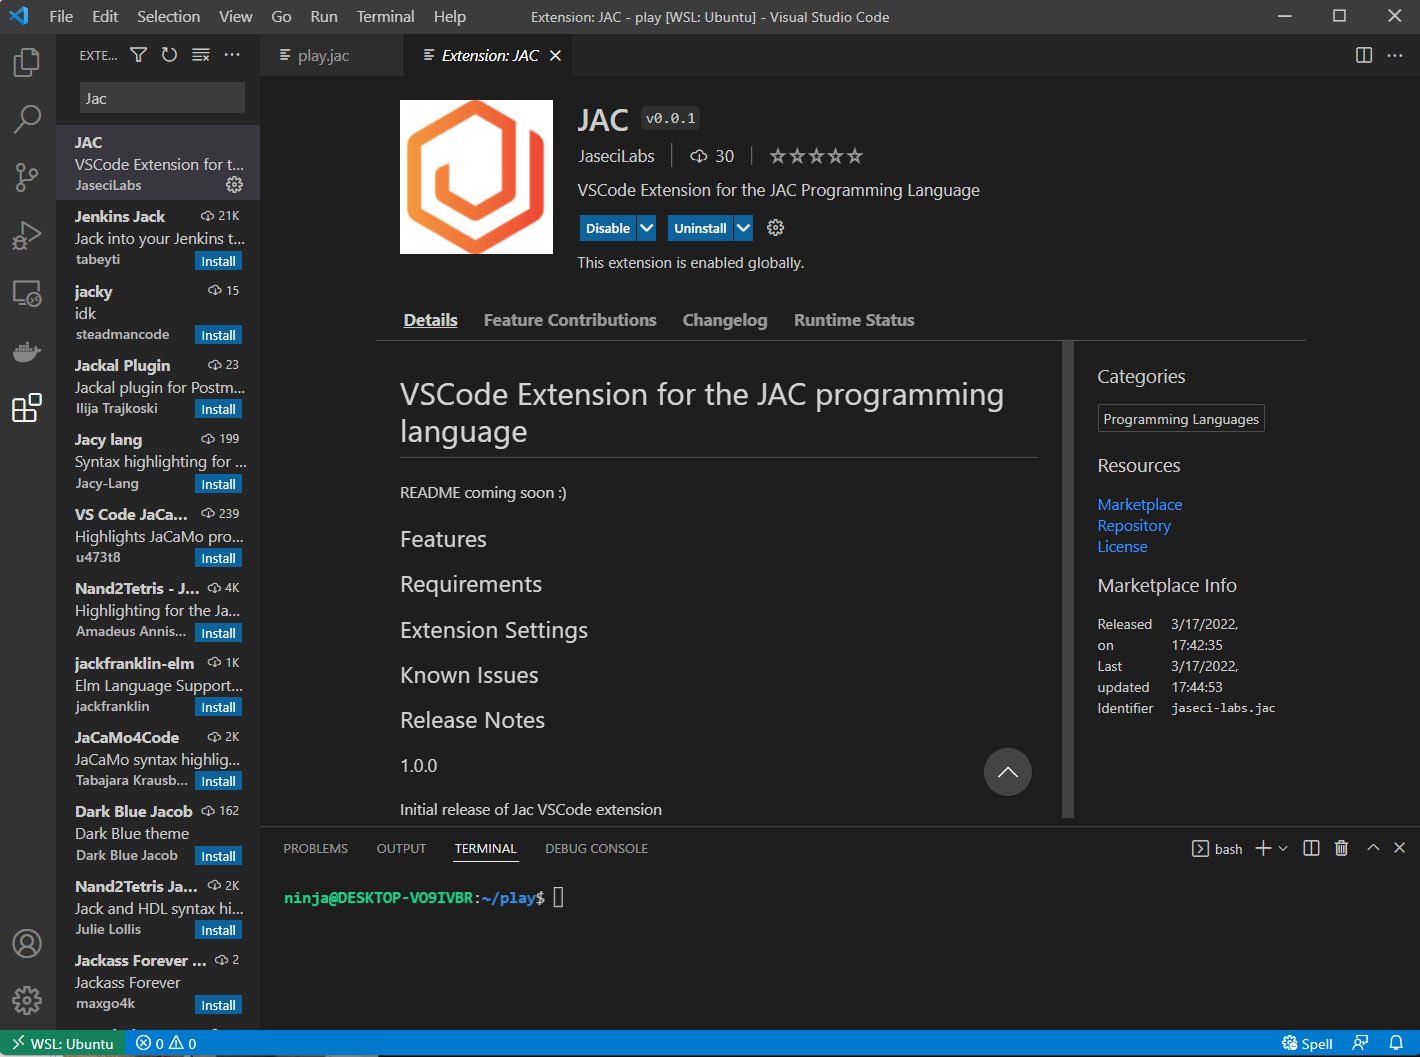
\includegraphics[width=.7\linewidth]{assets/images/vscode_jac_plugin.png}
    \caption[]{The Wonderful Jac Language extension in VSCode.}
    \label{fig:vscode_jac}
\end{figure}

\par
In VSCode, you can search for and install the Jac language extensions as per Figure~\ref{fig:vscode_jac}. As you can see, at the time I clipped this image, its quite new and doesn't really have a readme. You won't need one, it just provides syntax highlighting for \texttt{.jac} files at the moment. But it makes Jac code look beautiful, so it's a must have.

\begin{nerd}
    ...Personally, find an Ubuntu flavored \gls{WSL} VSCode environment to be the way to go these days. In a past life I was a 100\% Mac person for it's Unix based foundation. But WSL got soooooo good, and I had to switch! (plus there is insufficient gaming goodness in Mac-land). Anyway, I digress...
\end{nerd}



\chapter{Rants}

% \section{Libraries Suck}
% \label{rant:librariessuck}
% \par
% Because they do.
% \par
% Still need more reasons?
% \par
% Well, if you don't already know, I'm not going to tell you.
% \par
% \dots
% \par
% Still there?
% \par
% \dots
% \par
% Fine, I'll tell you.
% \begin{enumerate}
%     \item They suck because they create dependencies for which you must have faith in the implementer of the library to maintain and keep bug free.
%     \item They suck because there are often at least 10 options to choose from with near exact features expressing slightly different idiosyncratic ways.
%     \item They suck because they suck.
% \end{enumerate}
% Don't get me wrong, we have to use libraries. I'm not saying go reimplement the wheel 15 thousand times over. But that doesn't mean they don't suck and should be avoided if possible. The best is to know your library inside and out so the moment you hit some suckitude you can pull in the library's source code into your own codebase and \gls{pwn} it as your own.

\section{Utilizing Whitespace for Scoping is Criminal (Yea, I'm looking at you Python)}
\label{rant:whitespacesucks}
\par
This whitespace debauchery perpetrated by Python and the like is one of the most perverse abuses of ASCII code 32 I've seen in computer science. It's an assault on the freedom of coders to decide the shape and structure of the beautiful sculptures their creative minds might want to actualize in syntax. Coder's fingers have a voice! And that voice deserves to be heard! The only folks that support this oppression are those in the 1\% that get paid on a per line of code basis so they can lean on these whitespace mandates to pump up their salaries at the cost of coders everywhere.
\par
``FREE THE PEOPLE! FREE THE CODE!''
\par
``FREE THE PEOPLE! FREE THE CODE!''
\par
``FREE THE PEOPLE! FREE THE CODE!''

\section{``Using `master' in Git is NOT Racist!'' by a black dude}
\label{rant:racistmaster}
\par
[Insert Rant Here]

\chapter{Full Jac Grammar Specification}
\label{fullgrammar}
\gramcode{jac.g4}{Full listing of Jac Grammar (antlr4)}

\bibliographystyle{plain}
\bibliography{book}
\end{document}
